%%
% The BIThesis Template for Bachelor Graduation Thesis
%
% 北京理工大学毕业设计(论文)第四章节 —— 使用 XeLaTeX 编译
%
% Copyright 2020-2021 BITNP
%
% This work may be distributed and/or modified under the
% conditions of the LaTeX Project Public License, either version 1.3
% of this license or (at your option) any later version.
% The latest version of this license is in
%   http://www.latex-project.org/lppl.txt
% and version 1.3 or later is part of all distributions of LaTeX
% version 2005/12/01 or later.
%
% This work has the LPPL maintenance status `maintained'.
%
% The Current Maintainer of this work is Huang Chenrui.
%%

\chapter{仿真实验验证}

第2章和第3章对DQN及其改进算法和基于DQN的决策器、控制器的网络结构和具体实现进行了分析,本章将对基于DQN的决策器和控制器进行实验验证。基于DQN算法的决策器使用Highway-Env作为实验仿真环境;基于DQN算法的控制器使用Metadrive作为实验仿真环境。决策器和控制器实验均对比DQN及其改进算法的影响,主要验证在两种仿真环境中,经过多次训练的DQN算法的收敛性和可行性,同时对比DQN算法的改进型Double DQN和Dueling DQN,对比每个episode中的行为值函数、总体奖励、平均奖励和损失函数(Loss)的差异,从而根据结果对DQN及其改进算法进行效果改进和优劣分析。

\section{基于DQN算法的决策器实验}\label{4.1基于DQN算法的决策器实验}

基于DQN算法的决策器使用Highway-Env作为实验仿真环境,搭建第3章所述的决策器神经网络,通过Pytorch的API对自动驾驶决策器进行实现。具体实现的代码已上传至Github中以便查阅\cite{highway-env-dqn}。

\subsubsection{实验参数}

\begin{table}[htbp]
    \caption{决策器网络参数}\label{决策器网络参数}
    \centering
    \renewcommand\arraystretch{1.5}
    \setlength{\tabcolsep}{7mm}{
    \begin{tabular}{cc}
    \hline
    参数                & 参数值    \\ \hline
    学习率$\alpha$       & 1e-3   \\
    折扣因子$\gamma$      & 0.9    \\
    贪心算法参数$\epsilon$ & 0.9    \\
    TD网络更新步数$N$       & 1000   \\
    经验回放库$D$          & 2000   \\
    经验回放库抽取批次$batch$  & 32     \\
    训练回合数$episode$    & 24000 \\ \hline
    \end{tabular}
    }
\end{table}

由于Highway-Env的实验环境较简单,对于DQN网络的经验回放,不需要容量太多的经验回放库便能学习得到目标,实验参数如表\ref{决策器网络参数}。同时,抽取的经验回放库批次更新的$batch\_size$采用32作为参数,兼顾了训练的精度和准确性。对于训练回合数$episode$,由于目的是探究DQN及其改进算法的收敛性和参数趋势,故采取较长时间的回合数进行训练。

\subsubsection{仿真效果}

在Highway-Env下,基于DQN算法的决策器仿真效果如图\ref{基于DQN算法的决策器仿真效果}所示,(a)$\sim$(f)代表仿真车辆完成自动驾驶避障的过程,仿真实验采用的方法是在一段定长的时段,随机生成车辆周围的障碍(此处是其他车辆)信息,一旦自我车辆撞击障碍则仿真环境结束并输出最终奖励。(a)$\sim$(f)的过程是在仿真过程中截取的一段典型的避障环节,可以看到,自我车辆能够自主地进行周围障碍的识别并躲避。

\begin{figure}[htbp]
    \vspace{13pt}
    \centering
    \subfigure[]{
        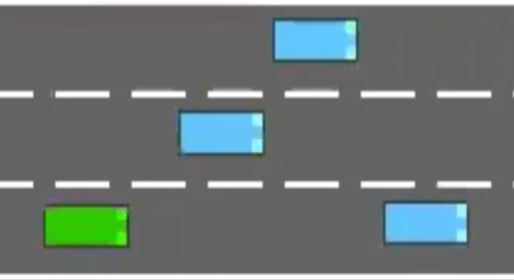
\includegraphics[scale=0.6]{images/chapter4/HighwayVideoSc/1.png}
        \label{subfig1}}
    % \hspace{0.01in} % 两图片之间的距离
    \subfigure[]{
        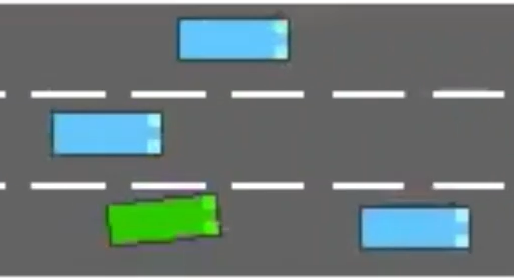
\includegraphics[scale=0.6]{images/chapter4/HighwayVideoSc/2.png}
        \label{subfig2}}
    \subfigure[]{
    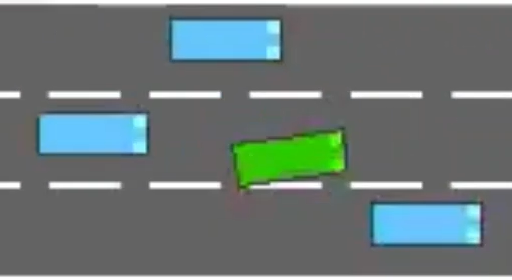
\includegraphics[scale=0.6]{images/chapter4/HighwayVideoSc/3.png}
    \label{subfig3}}
    \subfigure[]{
    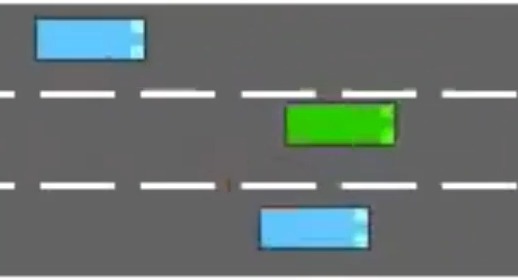
\includegraphics[scale=0.6]{images/chapter4/HighwayVideoSc/4.png}
    \label{subfig4}}
    \subfigure[]{
    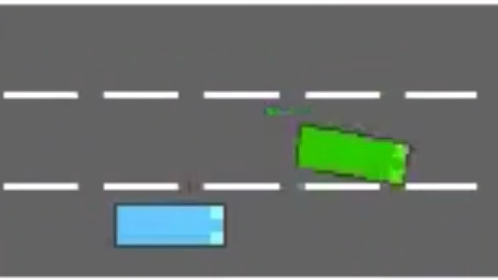
\includegraphics[scale=0.6]{images/chapter4/HighwayVideoSc/5.png}
    \label{subfig5}}
    \subfigure[]{
    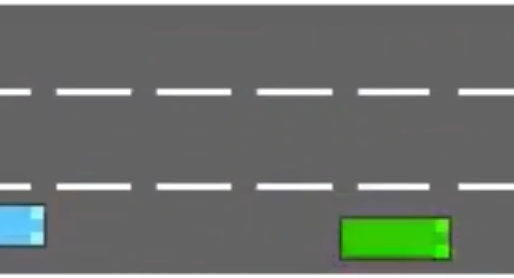
\includegraphics[scale=0.6]{images/chapter4/HighwayVideoSc/6.png}
    \label{subfig6}}
    \caption{基于DQN算法的决策器仿真效果}\label{基于DQN算法的决策器仿真效果} 
\end{figure}

以上行驶过程是智能体经过10000次训练达成的结果,经过10000次的训练,自动驾驶车辆基本学会了主动换道与避障的策略,能够使自动驾驶车辆在一定的时间段内稳定行驶到终点。下面将通过具体的数据对DQN算法的输出进行分析。

\subsubsection{基于DQN算法的决策器收敛性}

在验证DQN算法的效果前,需要判定DQN算法的收敛性。图\ref{DQN算法的Loss}表示的是整个训练过程中损失函数Loss的变化,此处以参数每更新10万次进行采样,损失函数Loss的值在0.02以下,而图\ref{DQN算法的Q值}显示的是DQN算法的Q值,在2万次的训练次数后总体趋近于8.5的区间内。

\begin{figure}[htbp]
    \vspace{13pt}
    \centering
    \subfigure[DQN算法的Q值输出]{
        \includegraphics[width=0.45\textwidth]{images/chapter4/HighwayPic/DQN_Q_value.png}
        \label{DQN算法的Q值}
    }
    % \hspace{0.01in} % 两图片之间的距离
    \subfigure[DQN算法的损失函数]{
        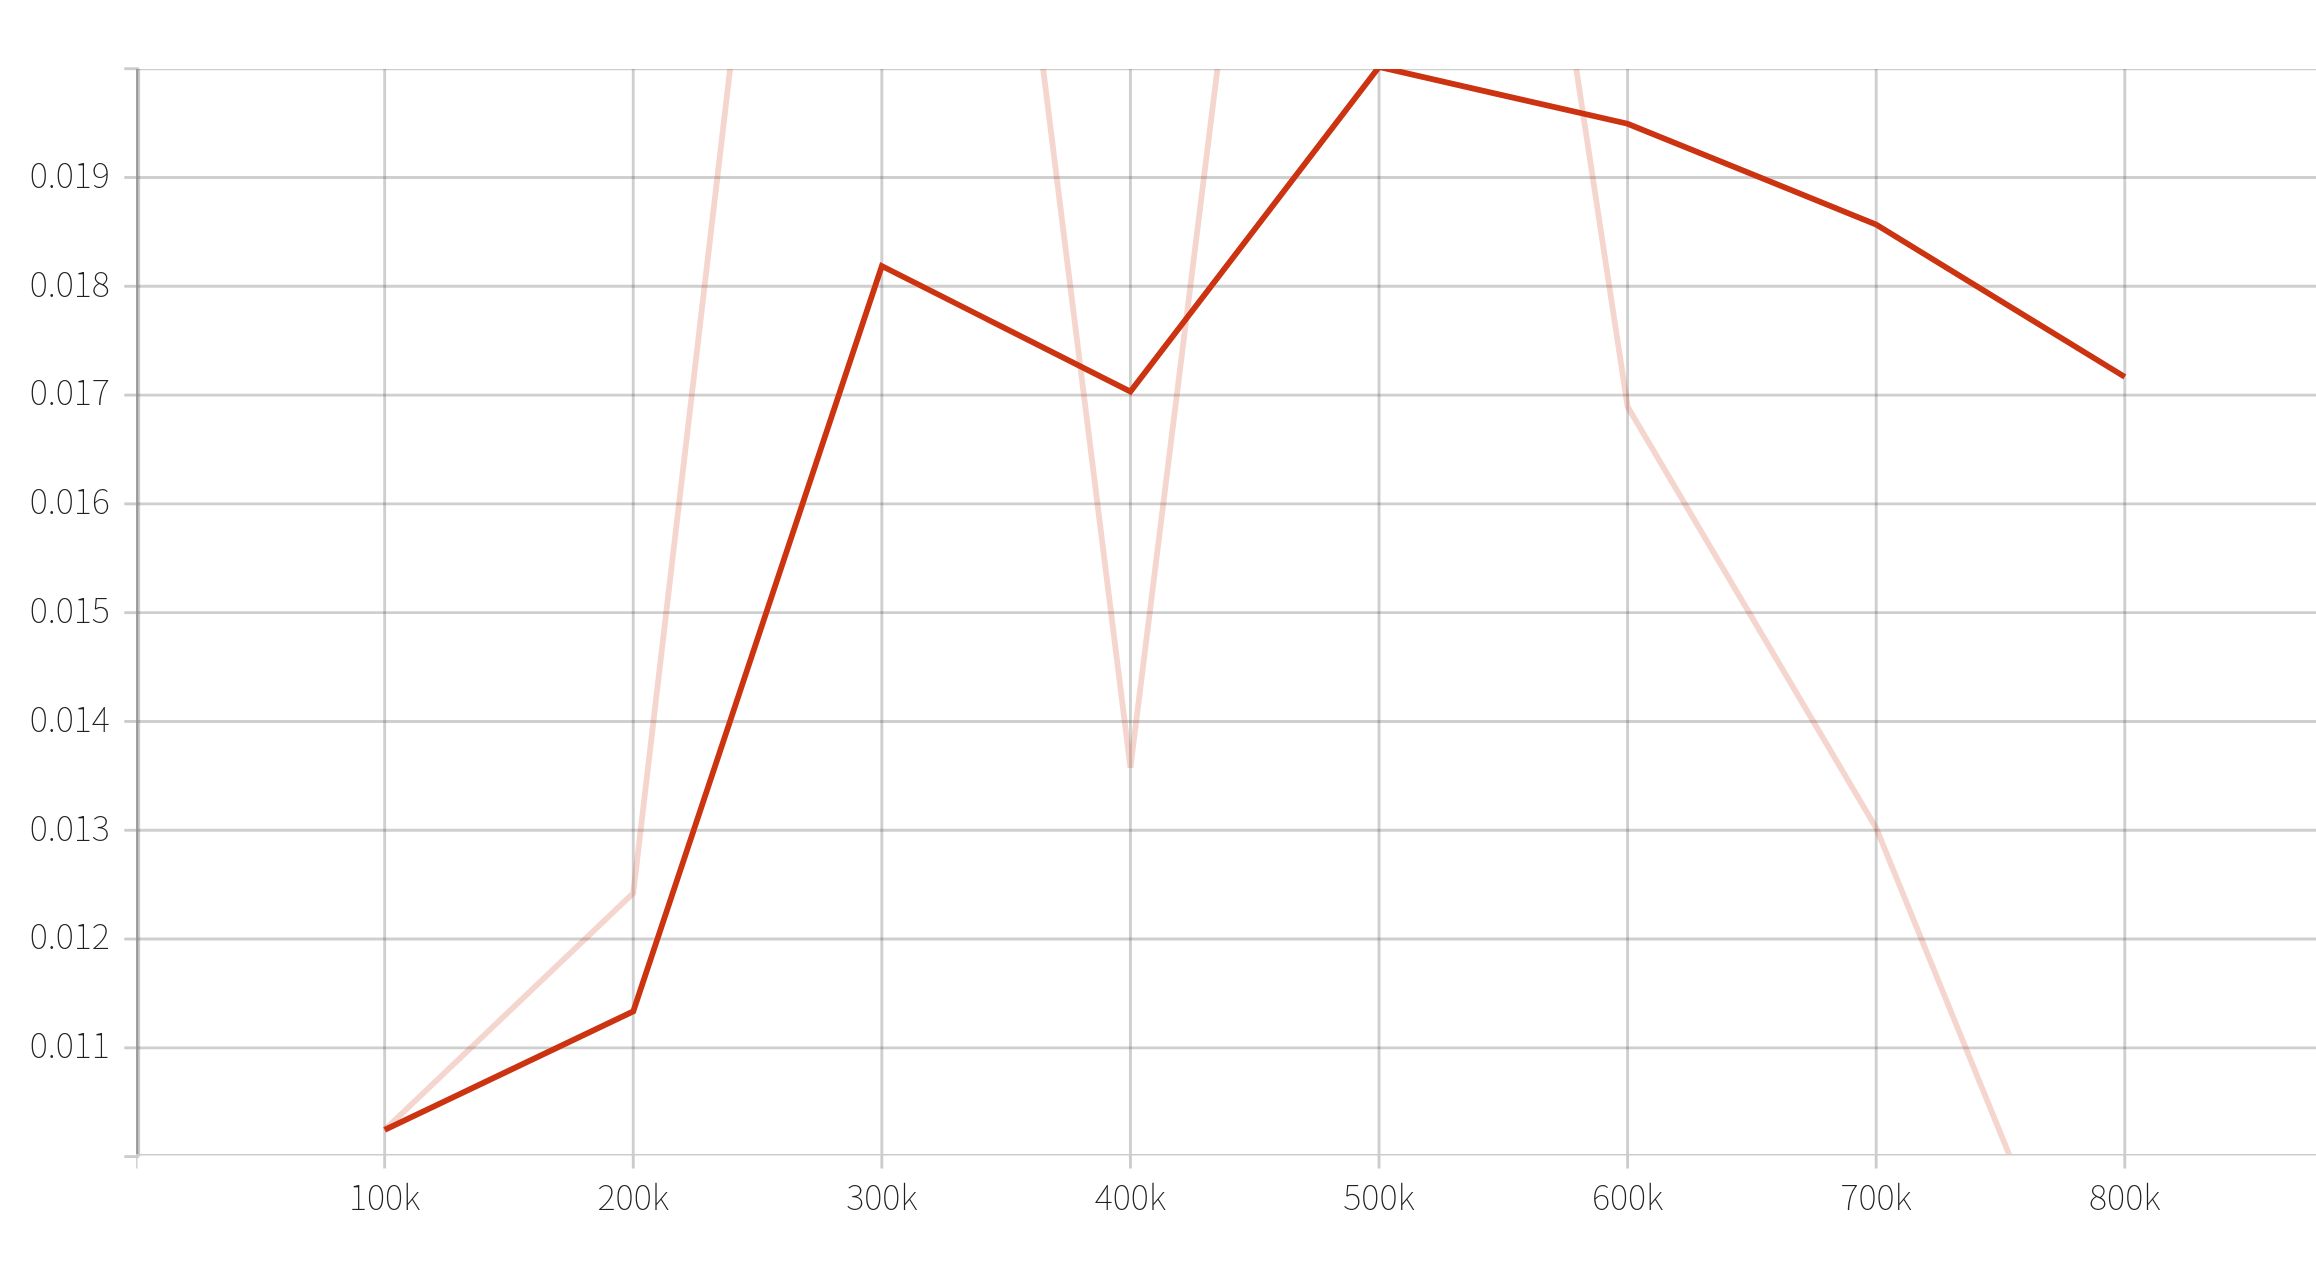
\includegraphics[width=0.45\textwidth]{images/chapter4/HighwayPic/DQN_Loss.png}
        \label{DQN算法的Loss}
    }
    \caption{DQN算法的收敛性}\label{DQN算法的收敛性} 
\end{figure}

\begin{equation}
    error = \frac{Loss}{Q\_Value} = \frac{0.02}{8.5} < 0.5\%
\end{equation}\label{dqn-decision-error}

根据图\ref{DQN算法的收敛性}所示,由于误差$<1\%$,此时可以判定DQN算法的收敛。

\subsubsection{基于DQN及其改进算法的决策器对比实验}

本实验验证了基于DQN、Double DQN和Dueling DQN算法的自动驾驶决策器,图\ref{DQN算法及其改进算法的收敛性对比}表示了三种算法的收敛性对比,其中红、蓝、橙三色曲线分别代表DQN、Double DQN、Dueling DQN的输出收敛情况。

\begin{figure}[htbp]
    \vspace{13pt}
    \centering
    \subfigure[DQN及其改进算法的Q值输出]{
        \includegraphics[width=0.45\textwidth]{images/chapter4/HighwayPic/Ave_Q_value.png}
        \label{DQN及其改进算法的Q值输出}
    }
    % \hspace{0.01in} % 两图片之间的距离
    \subfigure[DQN及其改进算法的损失函数]{
        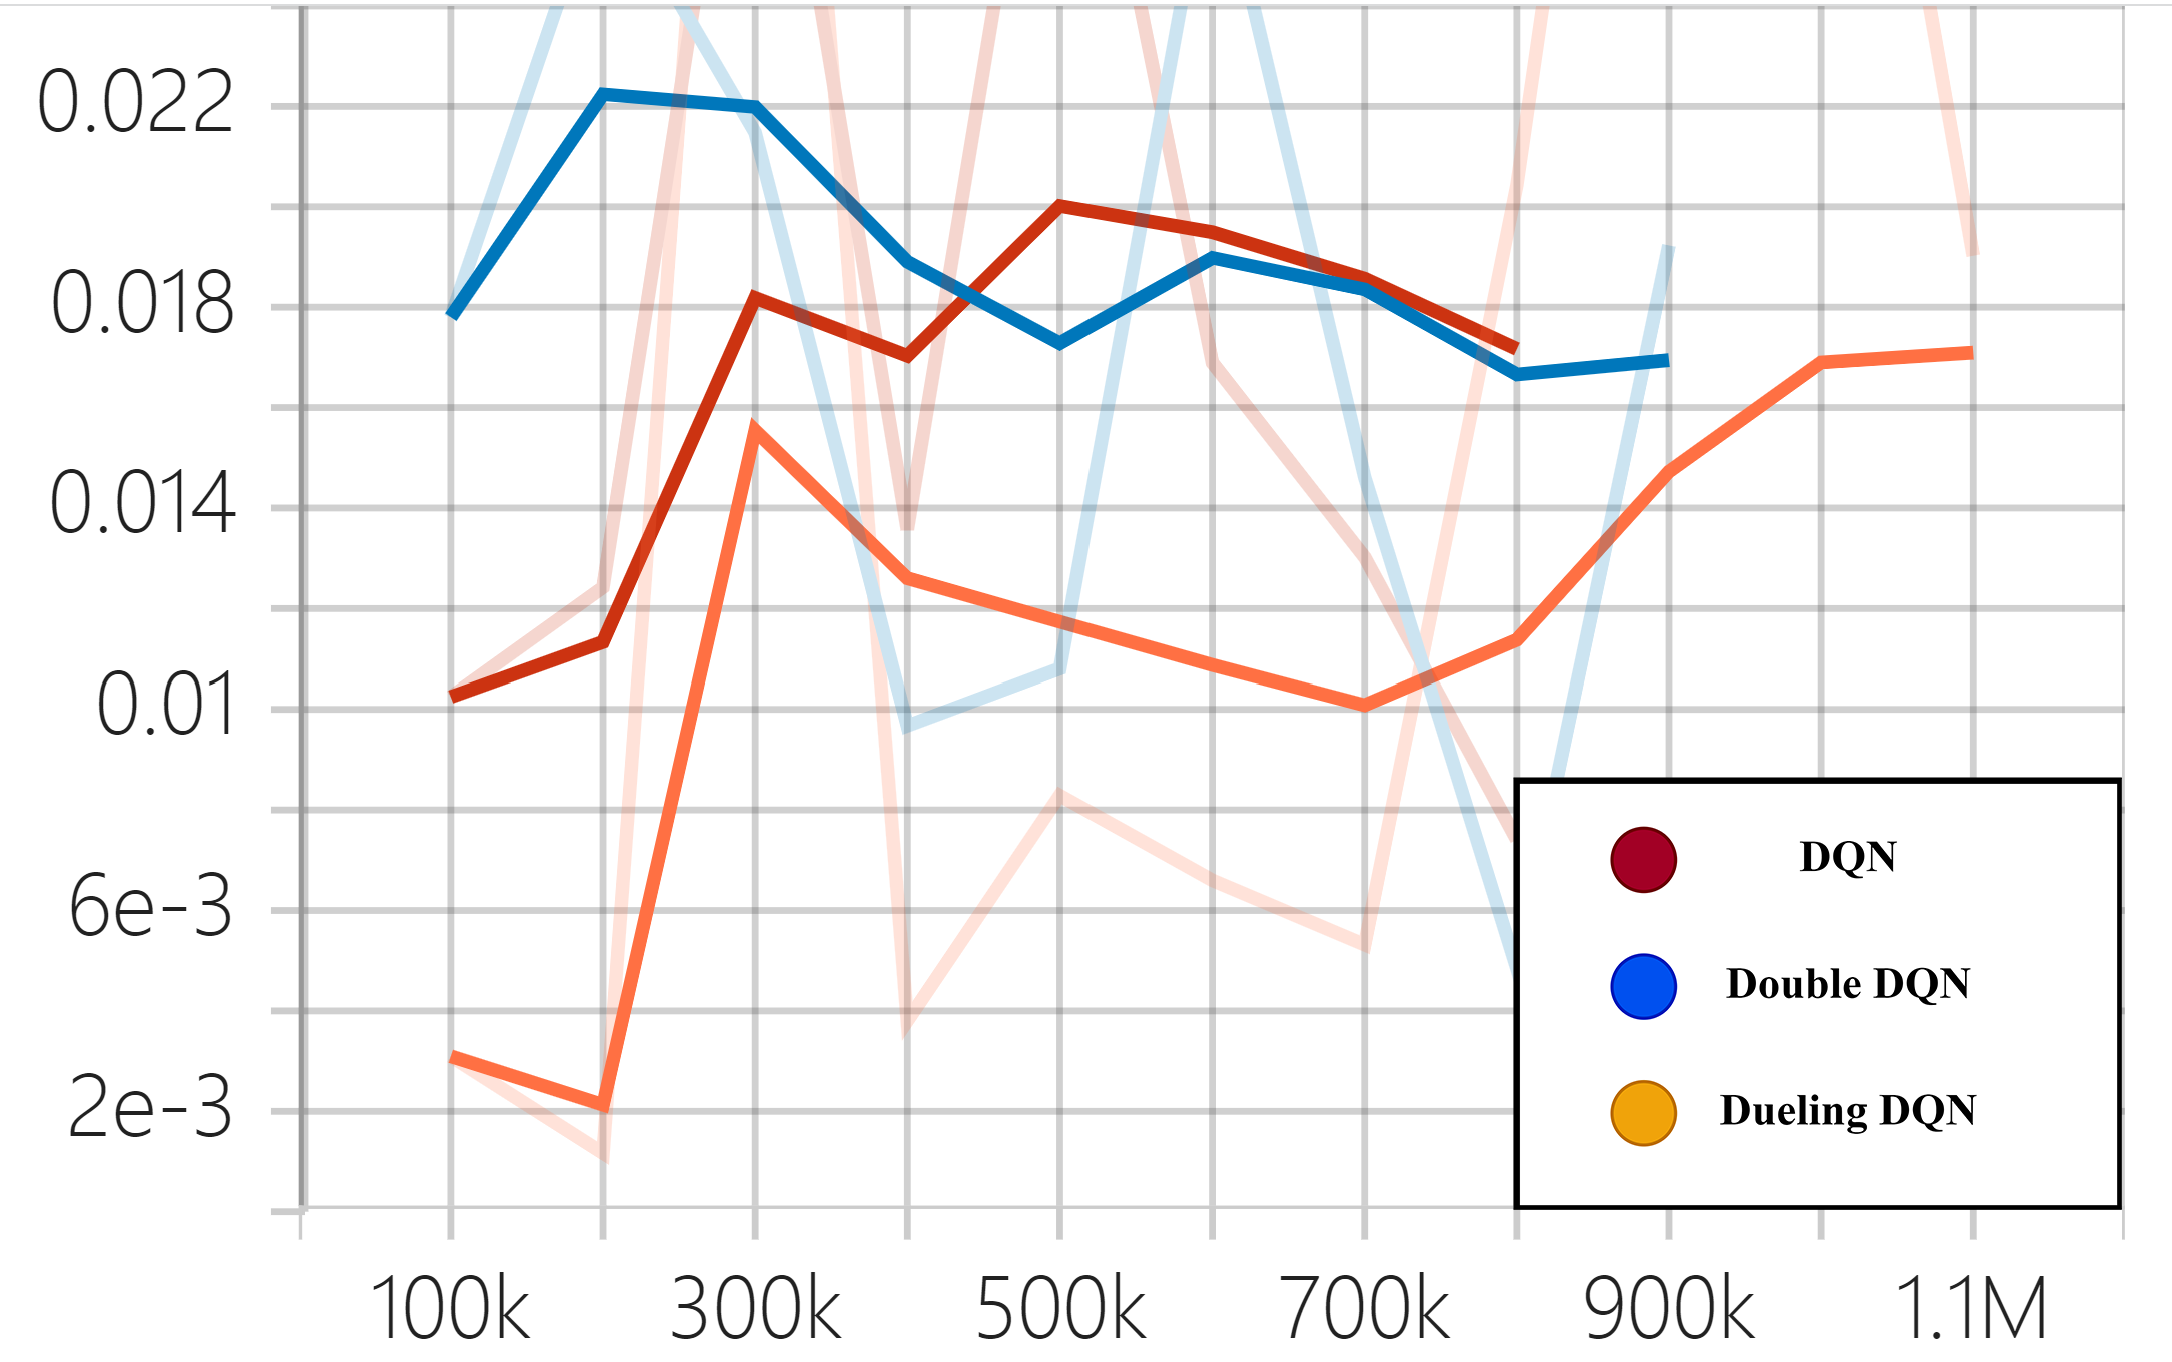
\includegraphics[width=0.45\textwidth]{images/chapter4/HighwayPic/Loss.png}
    }
    \caption{DQN算法及其改进算法的收敛性对比}\label{DQN算法及其改进算法的收敛性对比} 
\end{figure}

根据式\ref{dqn-decision-error}所示,由于Double DQN和Dueling DQN输出的Q值与损失函数与DQN差异不大,故三种算法在实验条件下均收敛。针对\ref{2.4改进的DQN算法}节提出的DQN存在的问题,由图\ref{DQN及其改进算法的Q值输出}能够看出,Double DQN算法解决了DQN算法的值函数过估计的问题,Dueling DQN算法相较于DQN算法也更早的进入了收敛状态。

\begin{figure}[htbp]
    \vspace{13pt}
    \centering
    \subfigure[每回合奖励值输出]{
        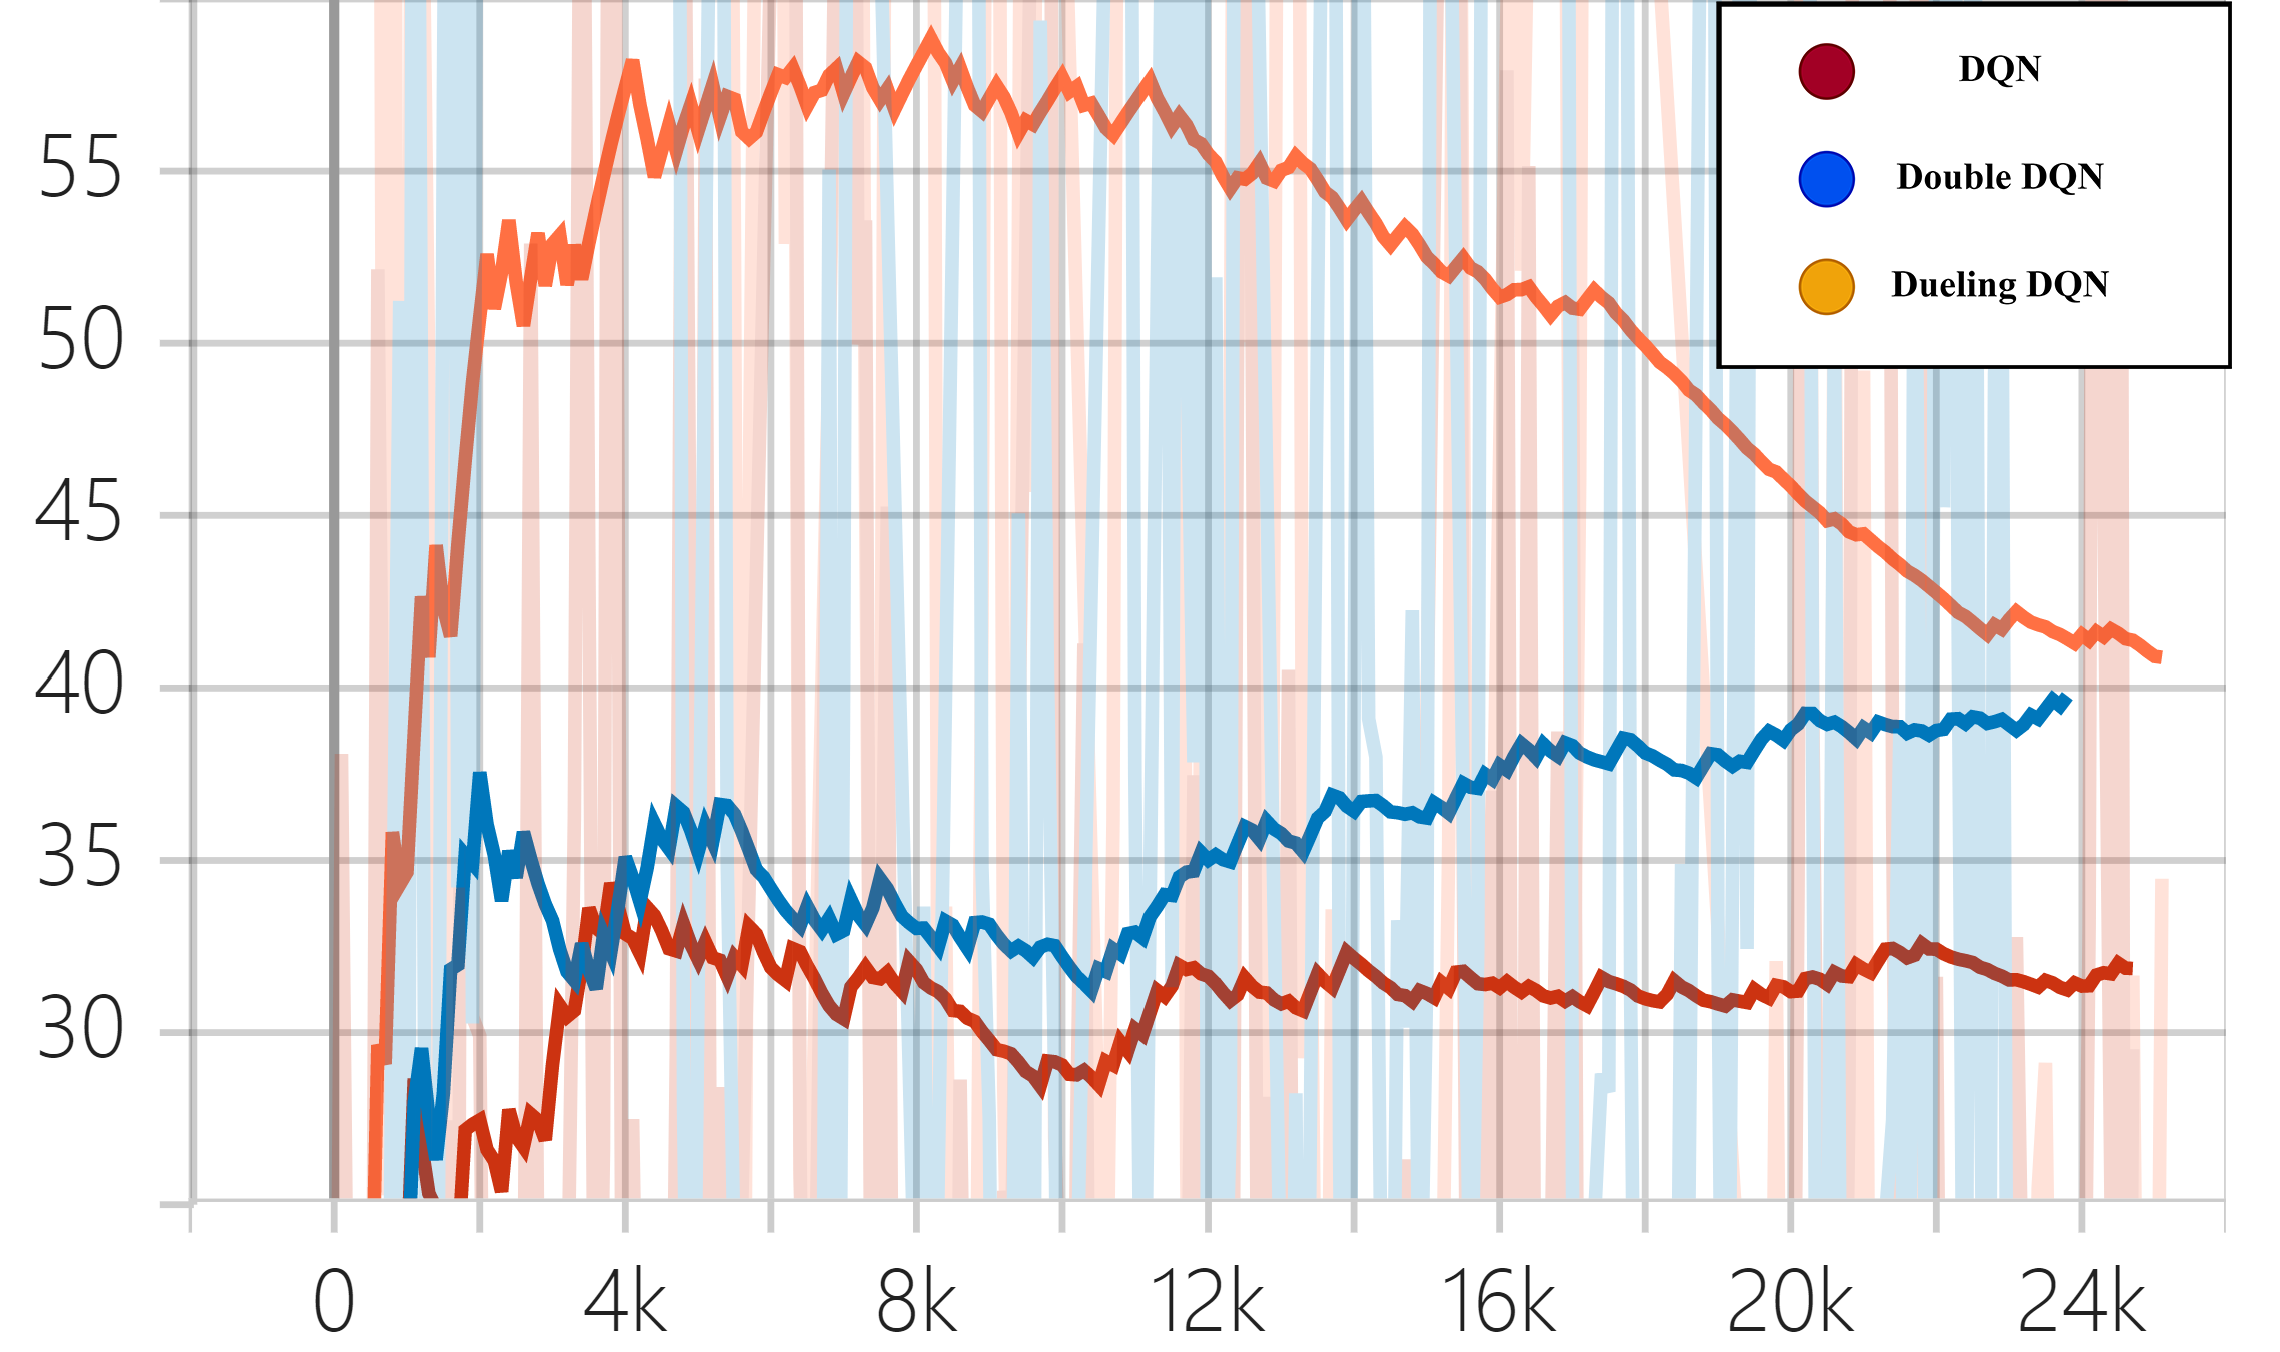
\includegraphics[width=0.45\textwidth]{images/chapter4/HighwayPic/Ep_r.png}
        \label{highway每回合奖励值输出}
        }
    % \hspace{0.01in} % 两图片之间的距离
    \subfigure[平均动作奖励值输出]{
        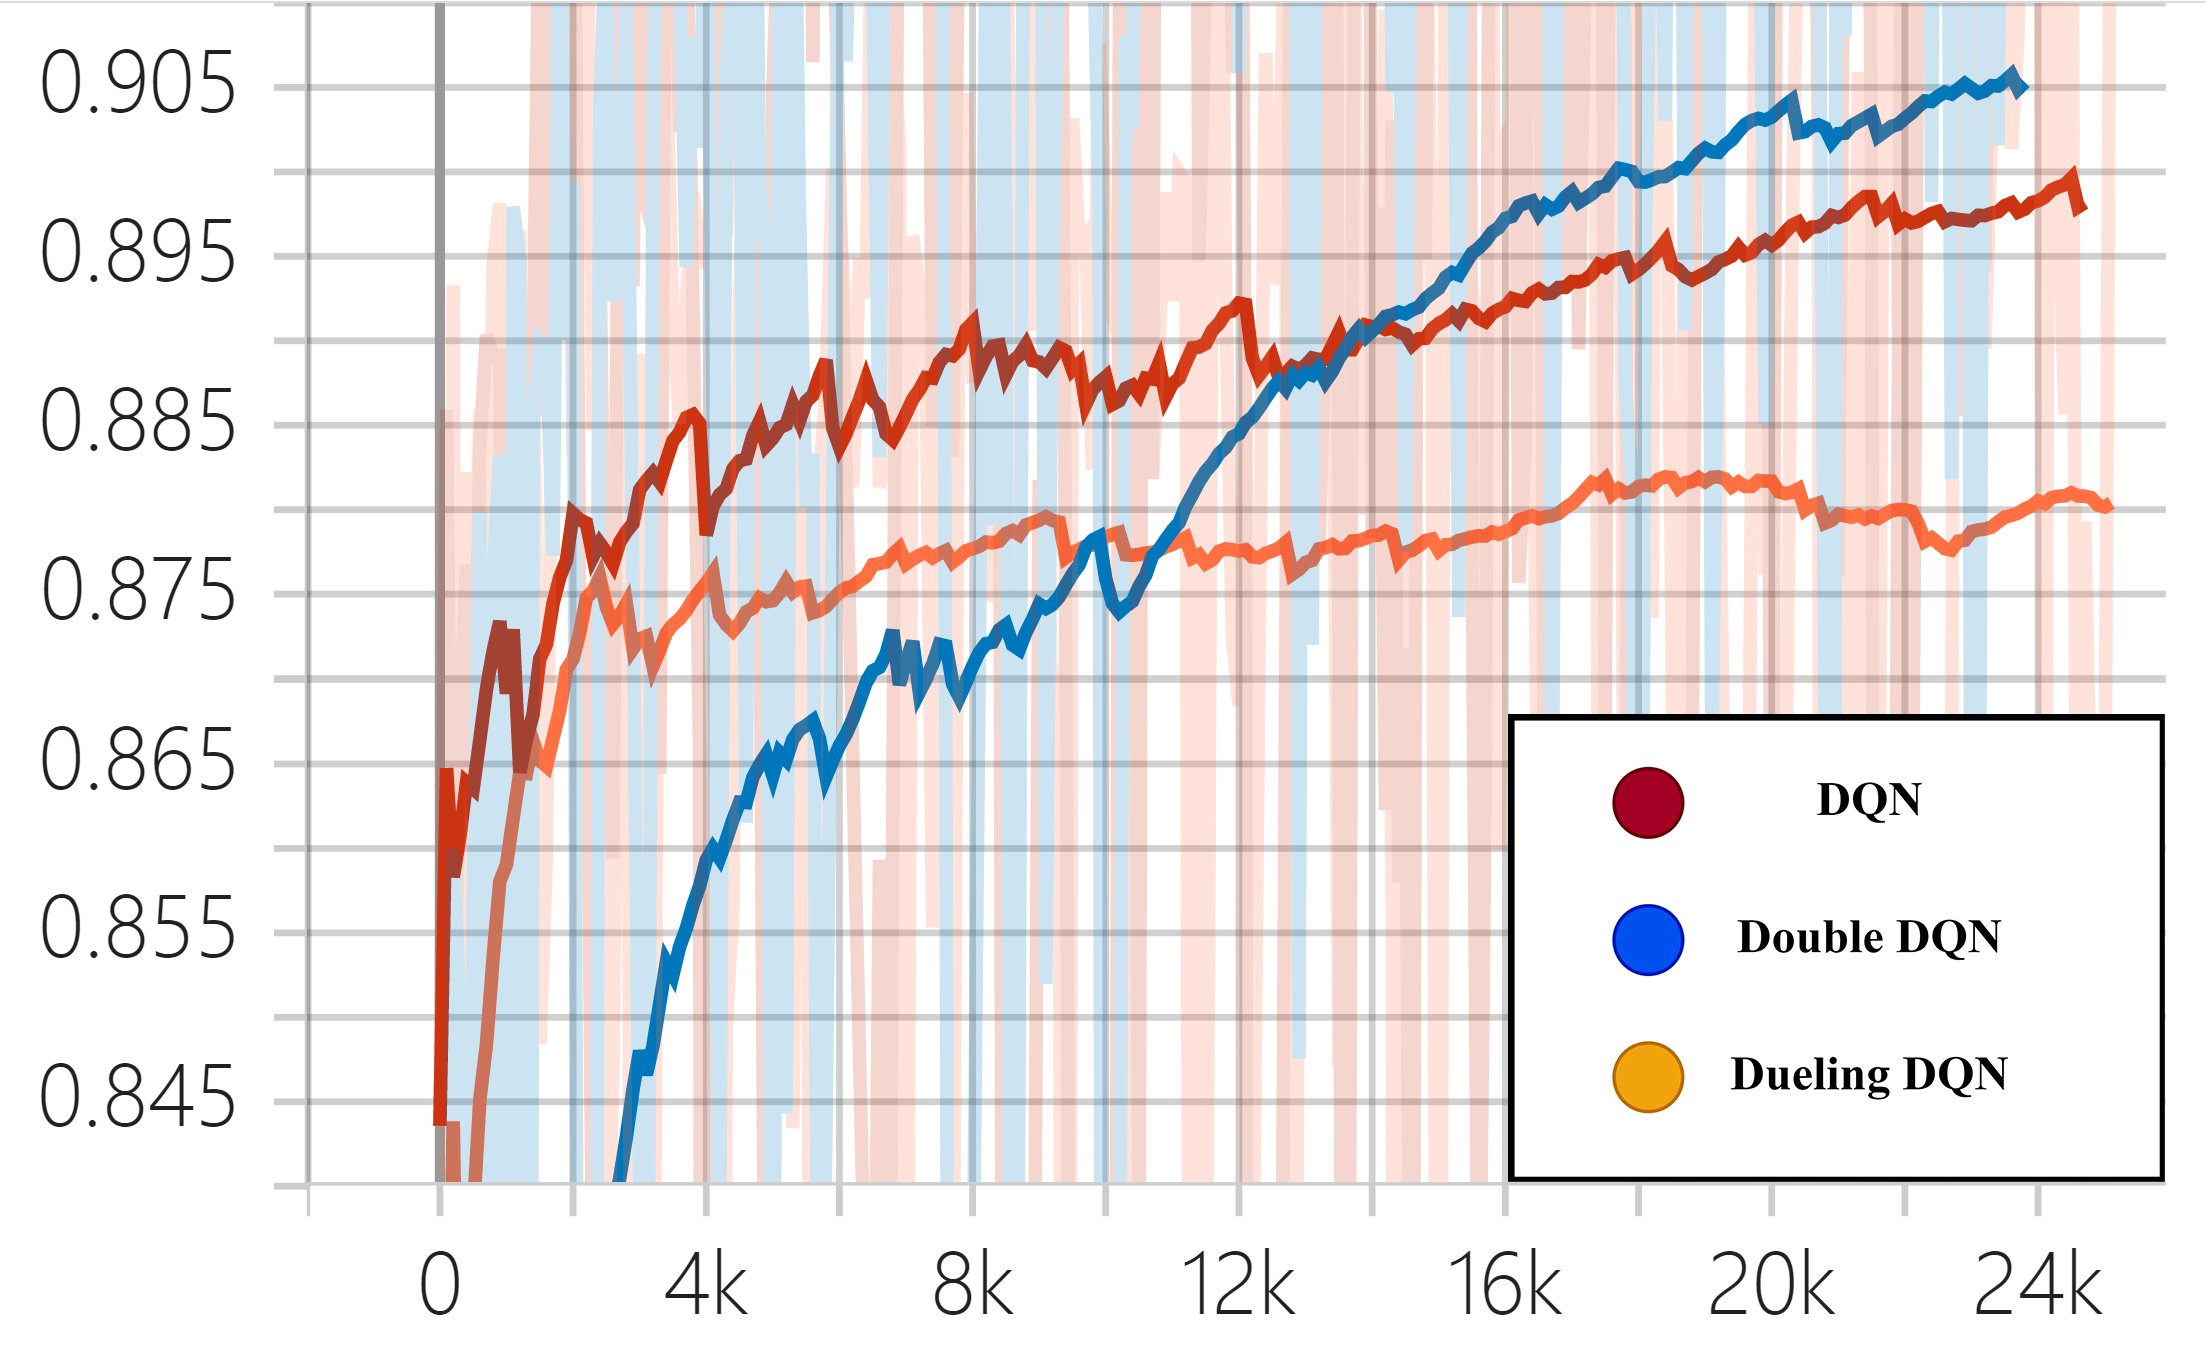
\includegraphics[width=0.45\textwidth]{images/chapter4/HighwayPic/Ave_r.png}
        \label{highway平均动作奖励值输出}
        }
    \caption{DQN算法及其改进算法的奖励值对比}\label{DQN算法及其改进算法的奖励值对比} 
\end{figure}

由图\ref{highway每回合奖励值输出}可知,Dueling DQN每回合得到的奖励值输出最高,在1万2千次训练后开始逐步下降至与Double DQN与DQN的奖励值输出接近,这是由DQN网络的实验参数(也称为超参数)和\ref{3.1.1仿真环境}节所表示的奖励函数式\ref{highway_reward}共同决定的,Dueling DQN在初始阶段学习到的策略在某个状态下能够得到较高的奖励函数,随着训练次数的提升和获取状态量的增加,Dueling DQN学习到了更加稳健的策略,奖励函数由原来的追求高速转向安全性的要求。

由图\ref{highway平均动作奖励值输出}可知,Double DQN的平均动作奖励值输出在1万2千次训练后开始逐步上升,Double DQN 分别采用不同的值函数来实现动作选择和动作评估,相对于最大化操作的值函数更新具有更加明显优势。

通过对以上仿真实验结果和数据的分析,DQN及其改进算法在Highway-Env仿真实验环境中完成自动驾驶决策任务能够得到收敛,对于平均动作奖励,Double DQN因其在动作选择和动作评估上的参数更新改进,能够得到相比于DQN和Dueling DQN更加良好的决策策略输出。

\newpage

\section{基于DQN算法的控制器实验}\label{基于DQN算法的控制器实验}

在基于DQN算法的决策器实验过程中,Double DQN算法对于平均动作奖励值输出有相对优异的表现,本节将DQN及其改进算法直接作用于动作输出,在不改变网络结构的情况下,重点关注Double DQN和其他DQN算法的对比实验效果。

基于DQN算法的控制器器使用Metadrive作为实验仿真环境,搭建第3章所述的控制器神经网络,通过Pytorch的API对自动驾驶控制器进行实现。具体实现的代码已上传至Github中以便查阅\cite{metadrive-dqn}。

\subsubsection{实验参数}

\begin{table}[htbp]
    \caption{控制器网络参数}\label{控制器网络参数}
    \centering
    \renewcommand\arraystretch{1.5}
    \setlength{\tabcolsep}{7mm}{
    \begin{tabular}{cc}
    \hline
    参数                & 参数值    \\ \hline
    学习率$\alpha$       & 1e-3   \\
    折扣因子$\gamma$      & 0.9    \\
    贪心算法参数$\epsilon$ & 0.9    \\
    TD网络更新步数$N$       & 1000   \\
    经验回放库$D$          & 50000   \\
    经验回放库抽取批次$batch$  & 32     \\
    训练回合数$episode$    & 100000 \\ \hline
    \end{tabular}
    }
\end{table}

由于Metadrive的状态输入涉及车身状态和导航信息等多样信息,对于DQN网络的经验回放,需要更多的经验回放库学习得到预期目标,实验参数如表\ref{控制器网络参数},经验回放库$D$容量扩大为50000,通过扩大经验回放库的方式使得智能体获取到更多的状态,避免智能体长时间获取单一状态集,失去算法的泛化性。对于训练回合数$episode$,为了得到稳定的DQN及其改进算法的参数趋势和应用性能,采取较长回合数进行训练,在实际的仿真实验环境中,经过约20000次的训练,DQN及其改进算法均已收敛,但得到稳定的参数仍需更多回合的训练次数,故将训练回合数设定为100000。

\newpage

\subsubsection{仿真效果}

在Metadrive的仿真环境下,图\ref{基于DQN算法的控制器仿真效果}体现的是基于Double DQN算法的控制器仿真效果,(a)$\sim$(f)代表仿真车辆完成自动驾驶路线循迹的过程,仿真实验采用的方法是在一段定长的时段,随机生成地图信息,一旦自我车辆触及黄线或逆向行驶,则仿真环境结束并输出最终奖励。(a)$\sim$(f)的过程是在仿真过程中截取的一段典型的循迹和换道环节,针对环形道路和直道等多样环境,自我车辆能够自主地进行周围信息的识别并较为稳定地输出轮转角和转矩$[steering, throttle]$,根据画面中的导航点信息,自主实现换道和车道保持循迹功能。

\begin{figure}[htbp]
    \vspace{13pt}
    \centering
    % \subfigure[]{
    %     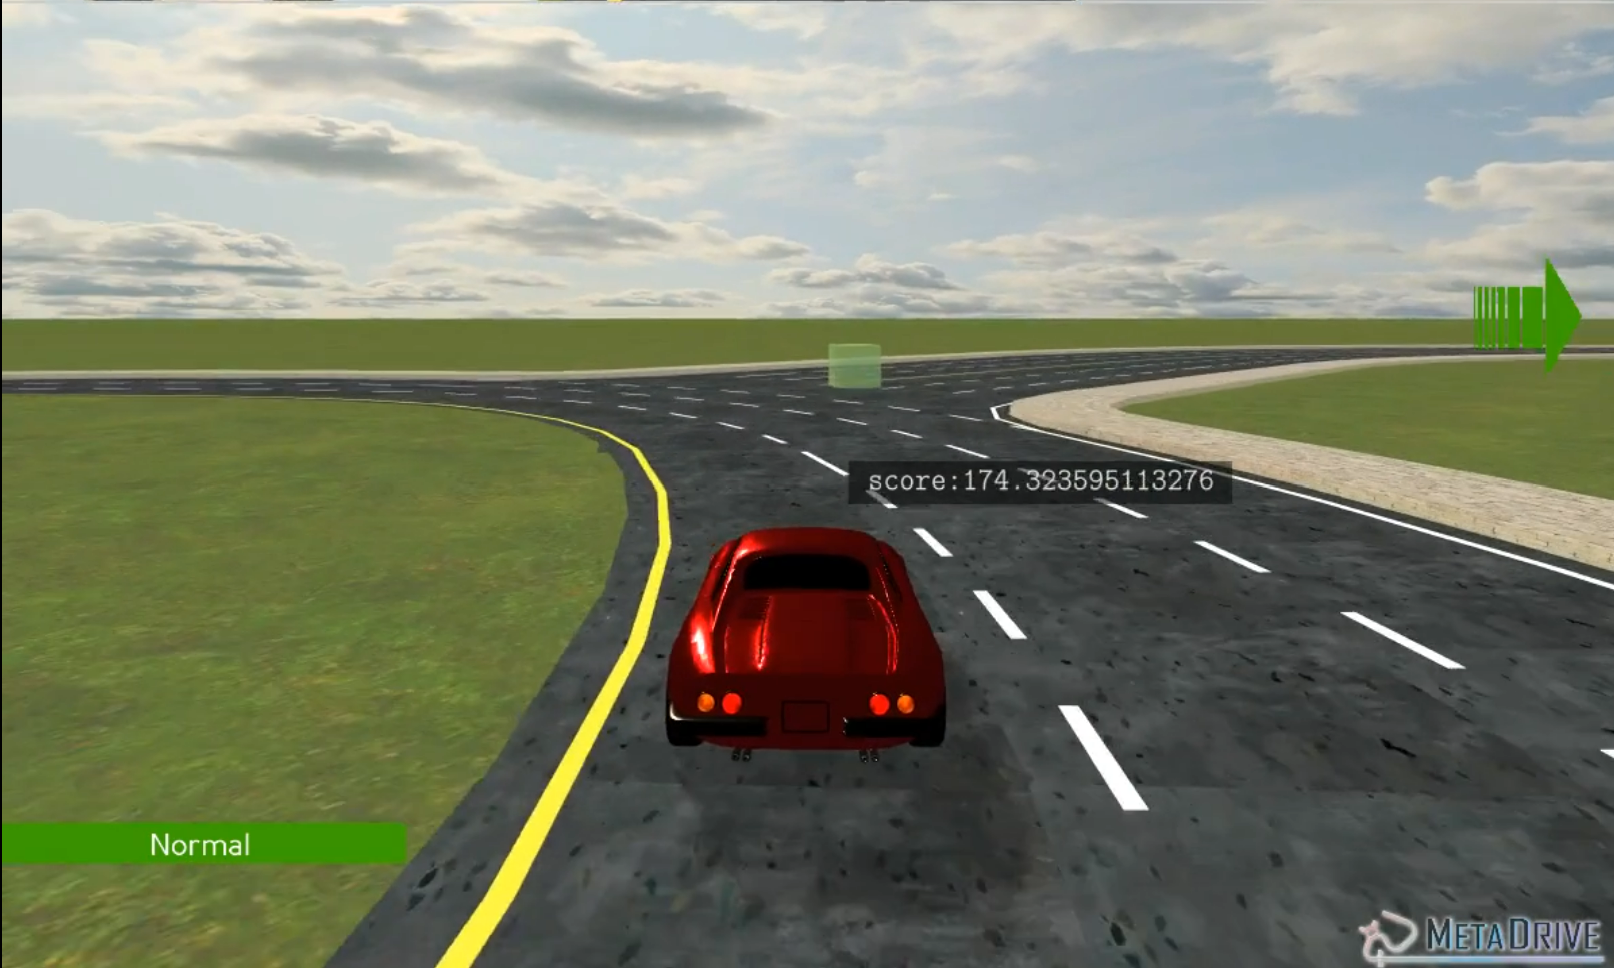
\includegraphics[width=0.2\textwidth]{images/chapter4/MetadriveVideoSc/1.png}
    %     }
    % \hspace{0.01in} % 两图片之间的距离
    \subfigure[]{
        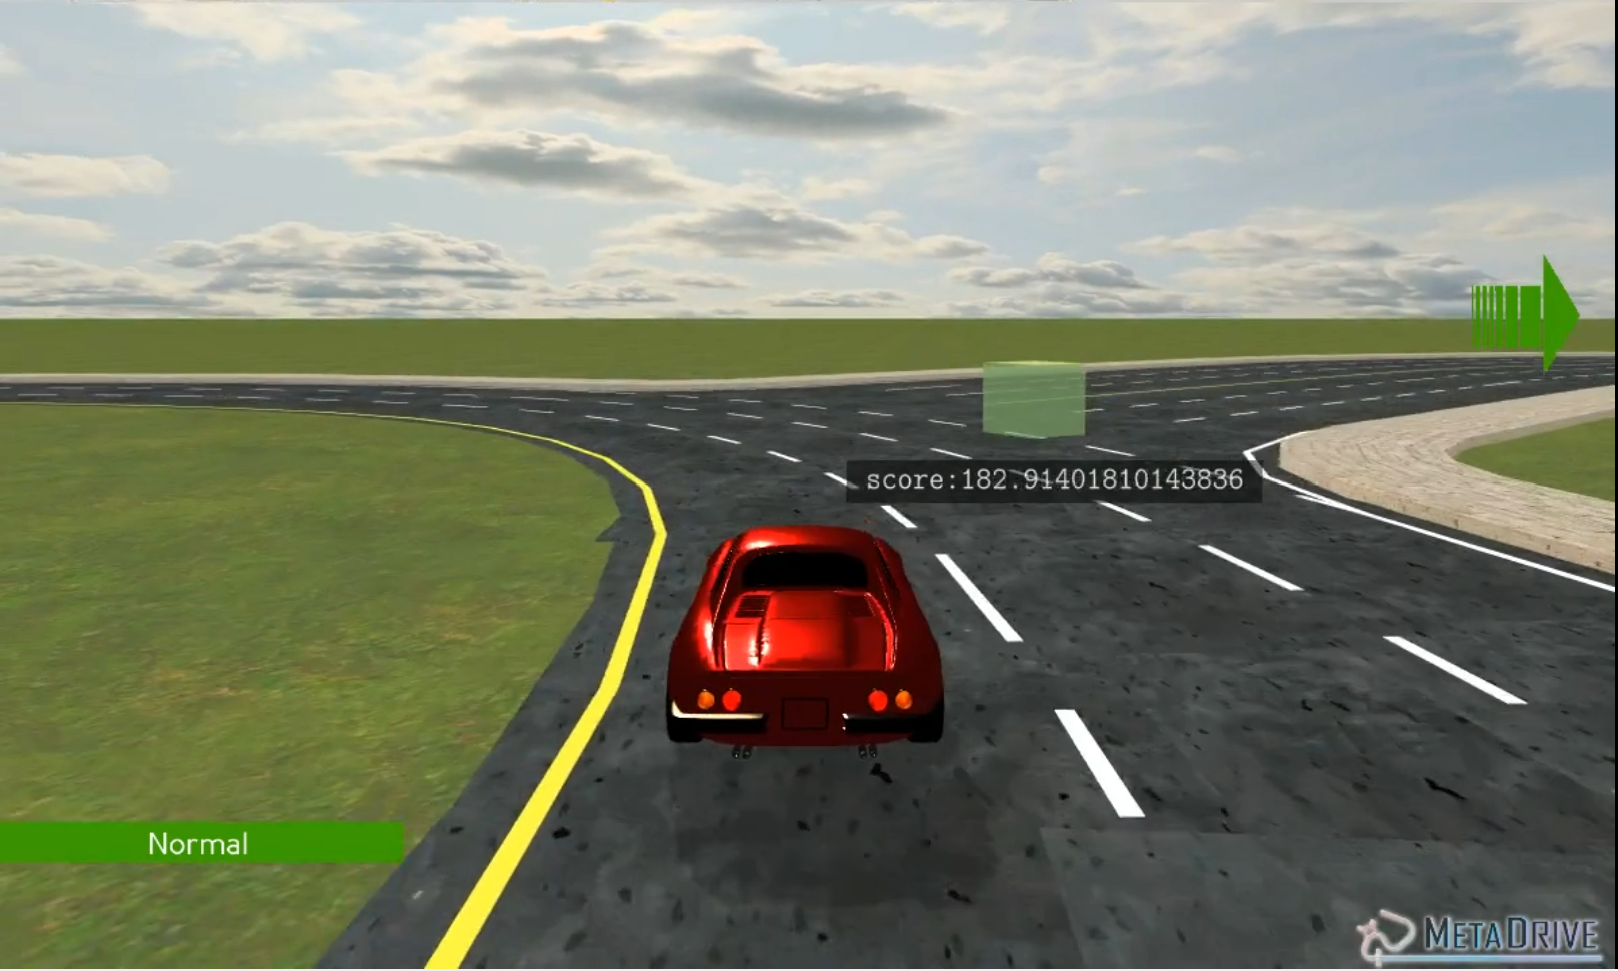
\includegraphics[width=0.3\textwidth]{images/chapter4/MetadriveVideoSc/2.png}
        }
    \subfigure[]{
    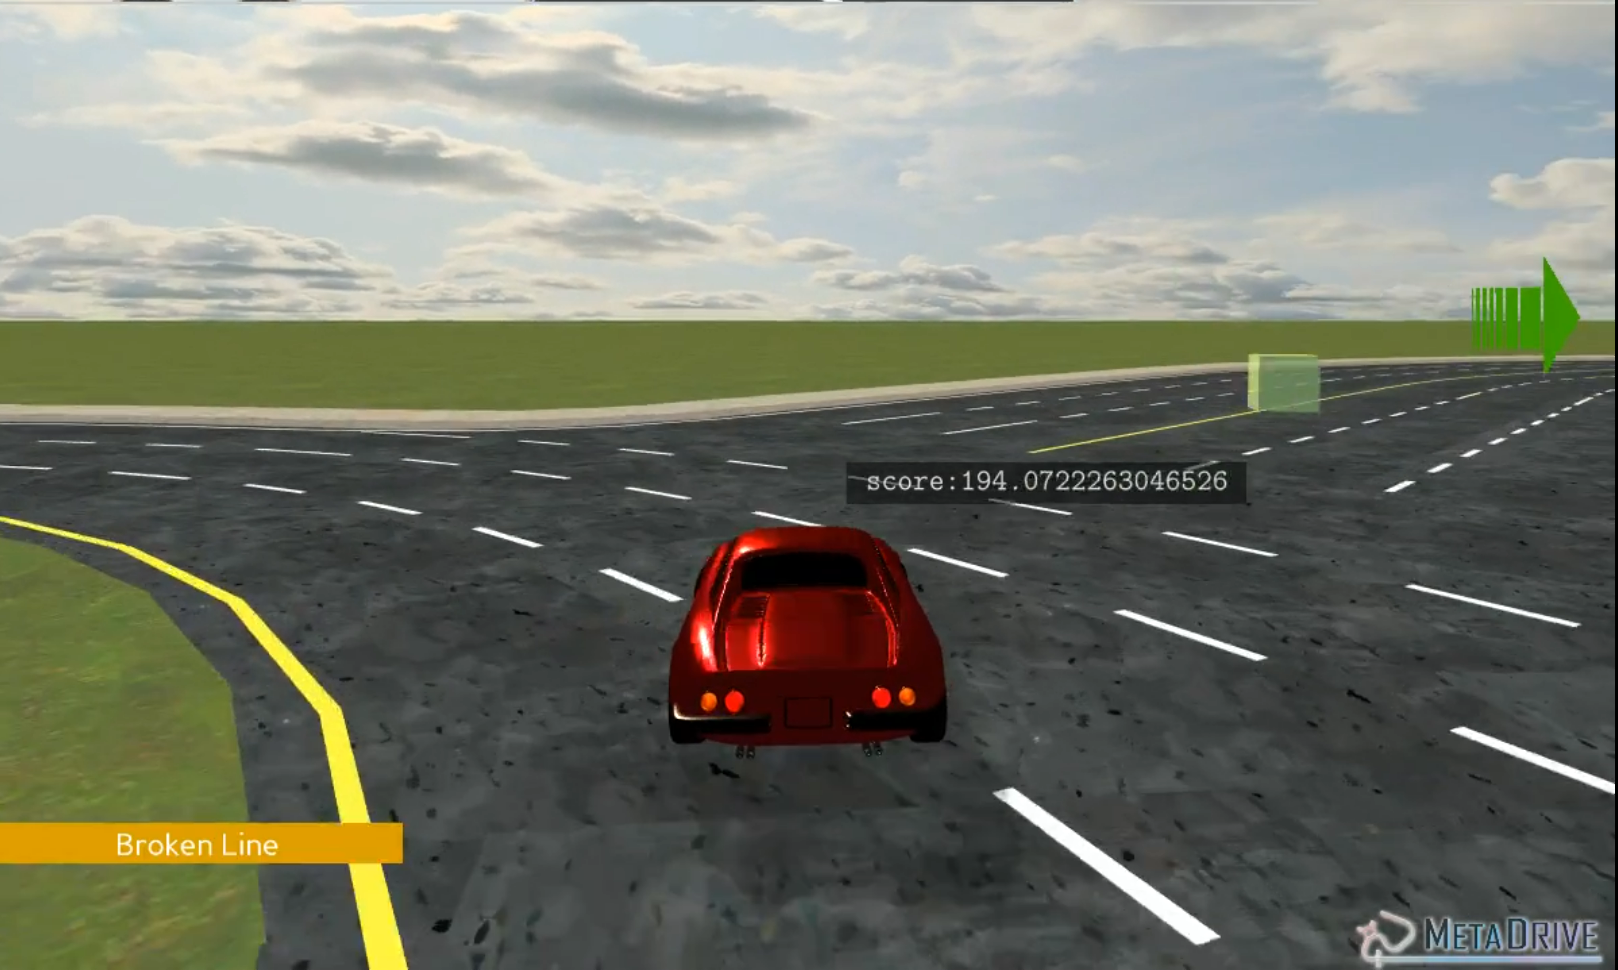
\includegraphics[width=0.3\textwidth]{images/chapter4/MetadriveVideoSc/3.png}
    }
    \subfigure[]{
    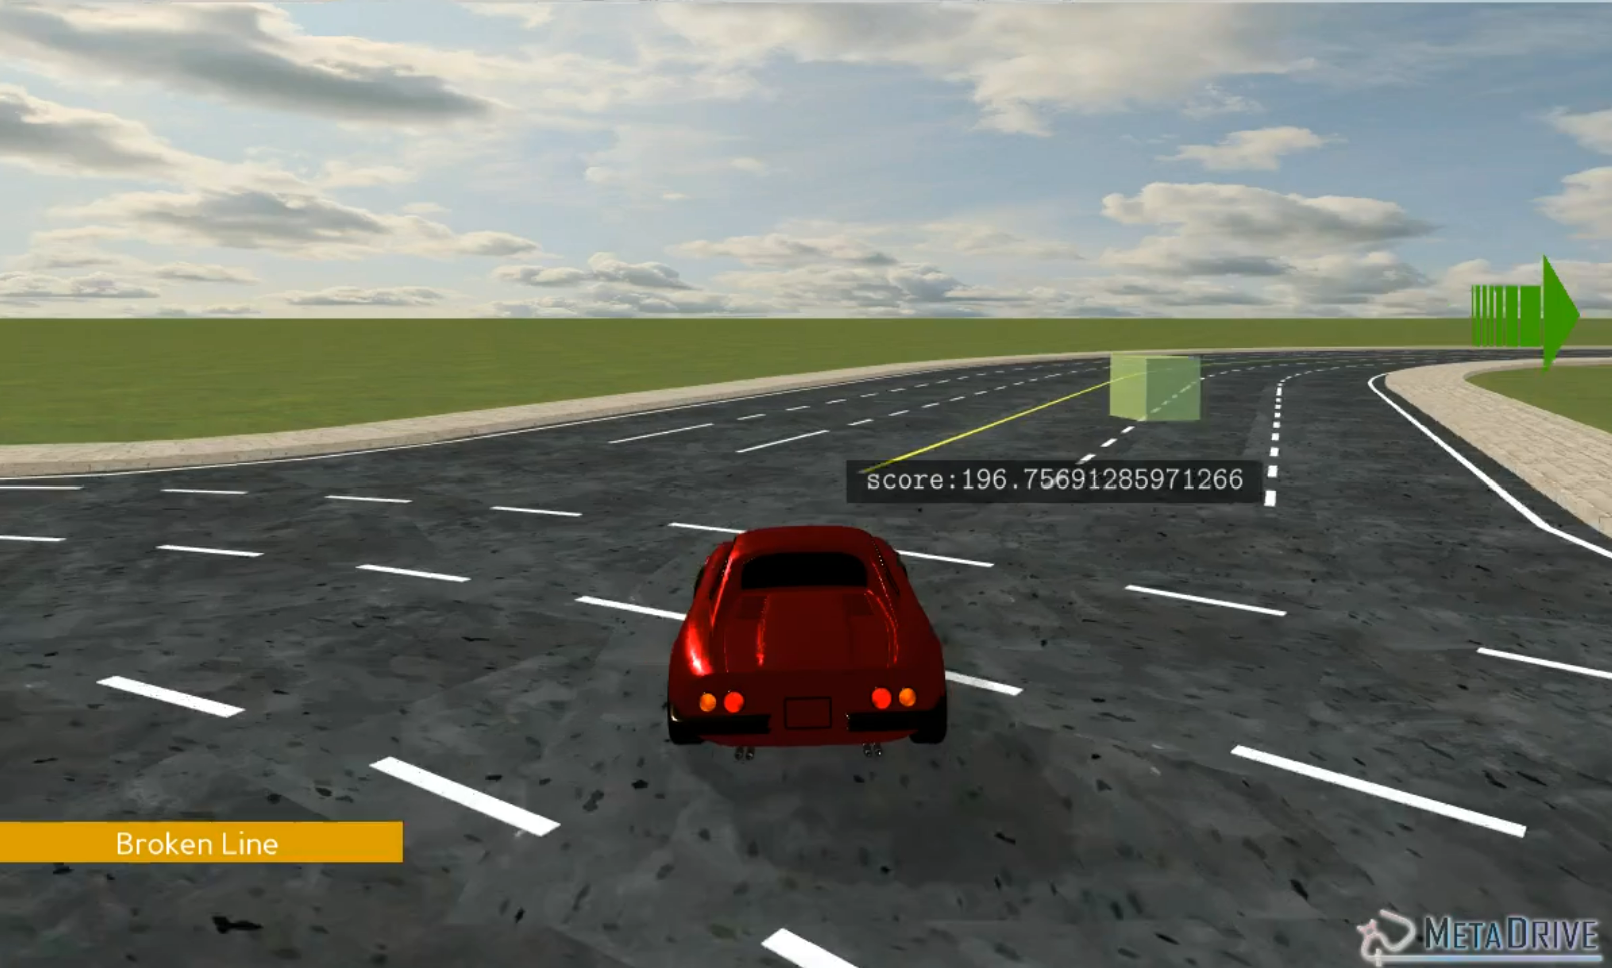
\includegraphics[width=0.3\textwidth]{images/chapter4/MetadriveVideoSc/4.png}
    }
    \subfigure[]{
    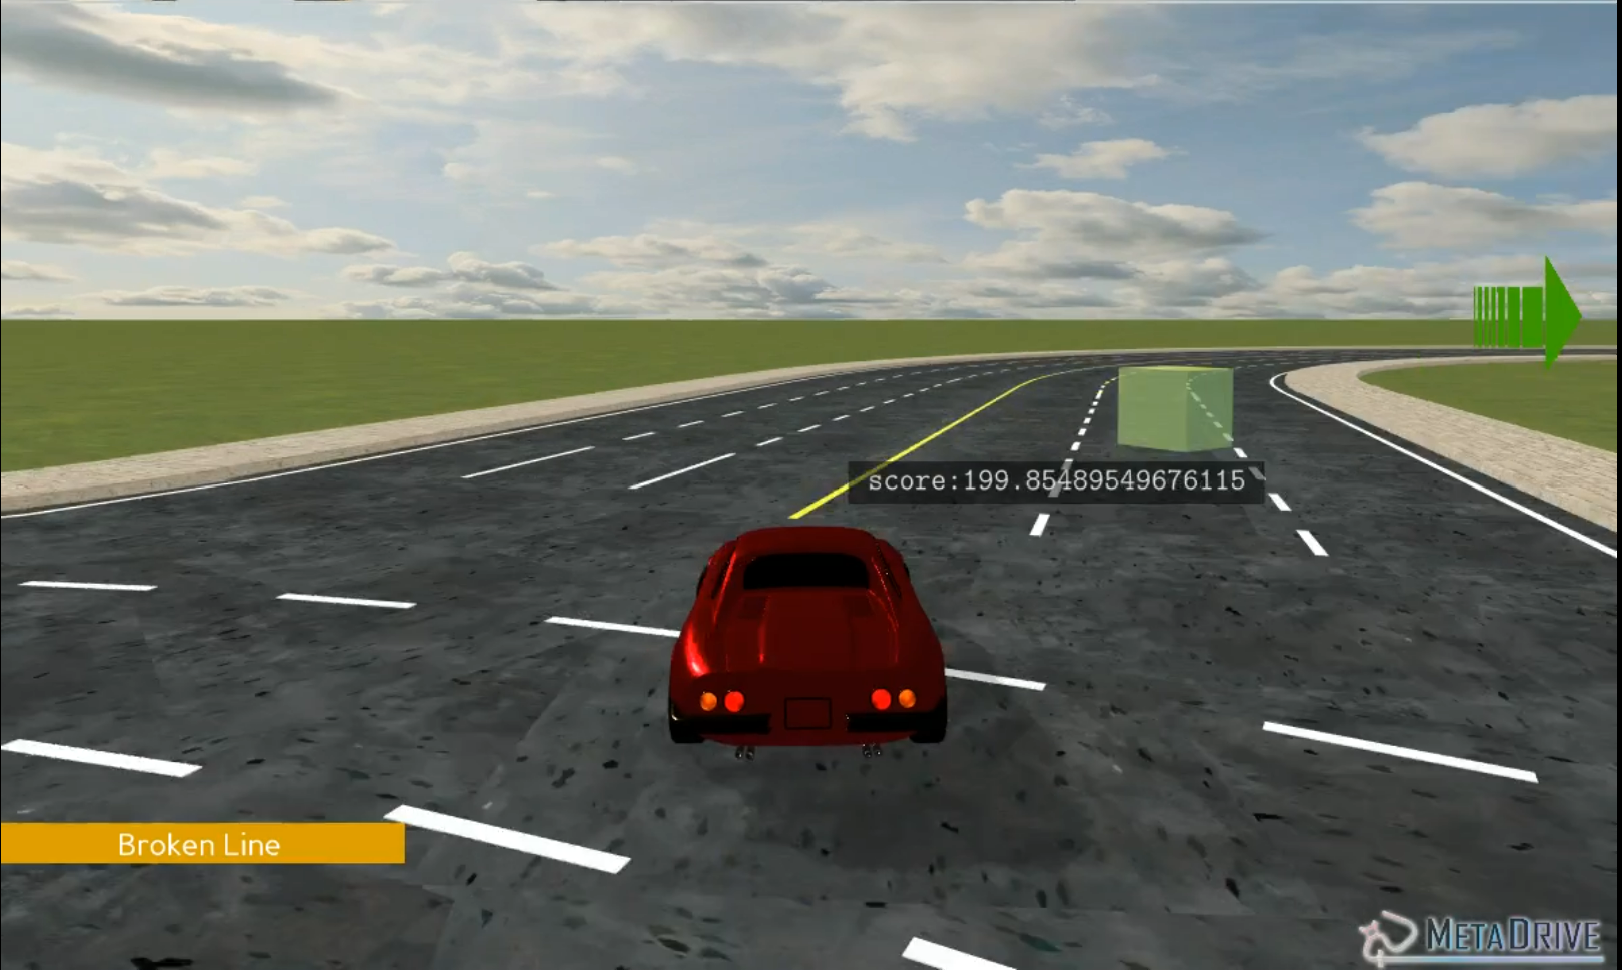
\includegraphics[width=0.3\textwidth]{images/chapter4/MetadriveVideoSc/5.png}
    }
    \subfigure[]{
    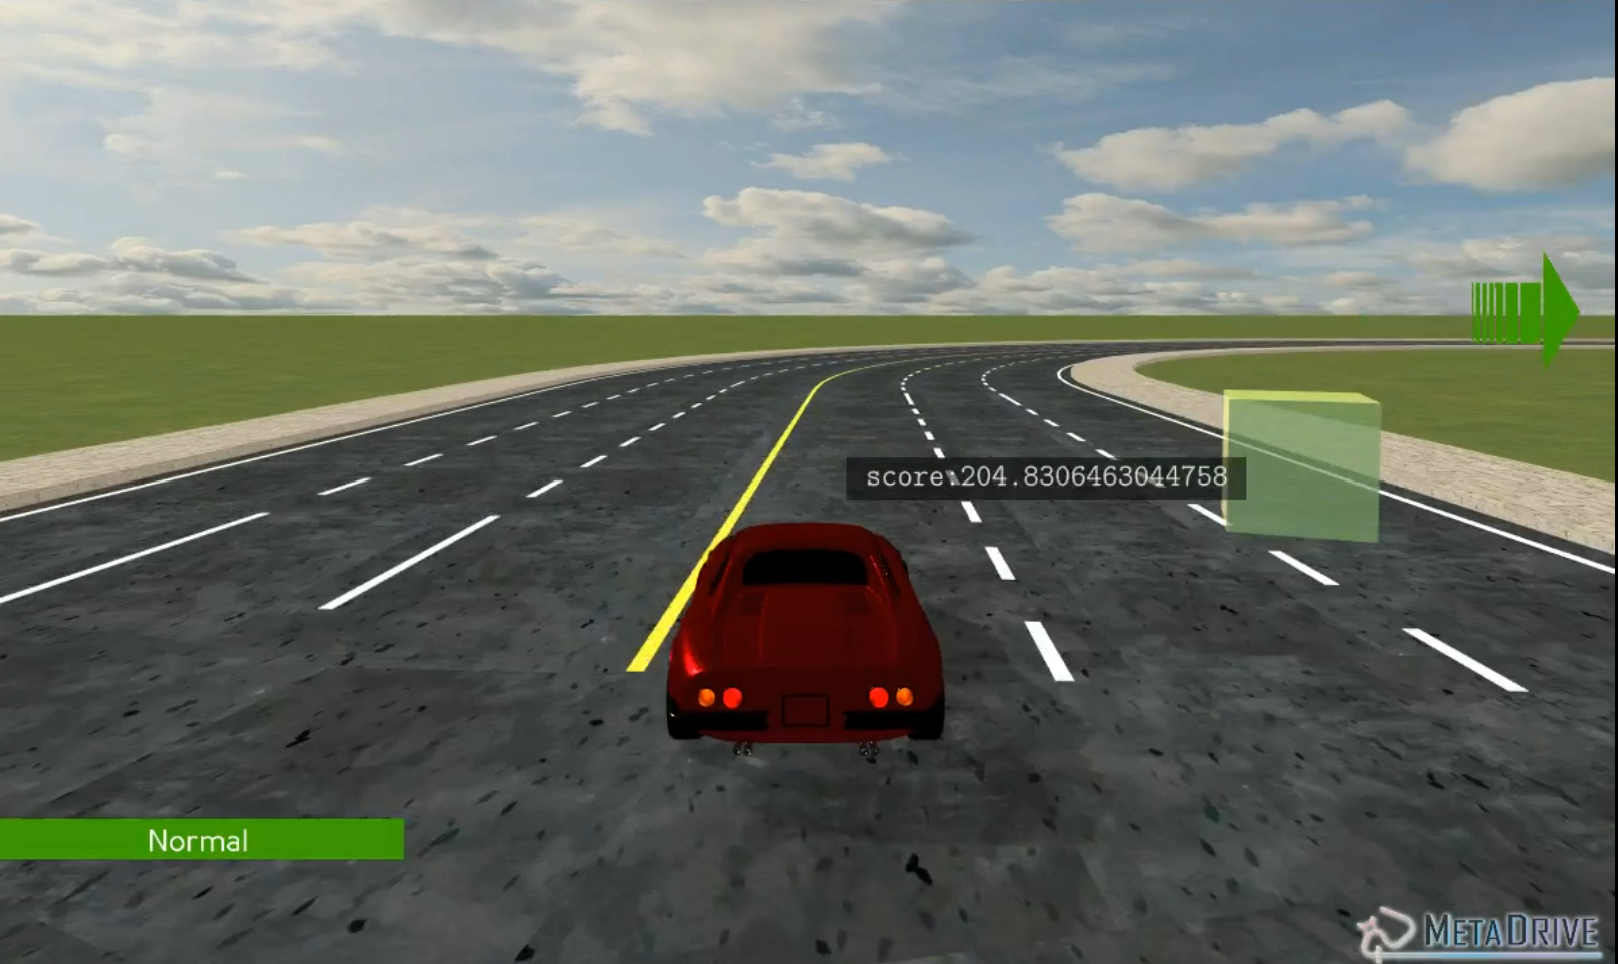
\includegraphics[width=0.3\textwidth]{images/chapter4/MetadriveVideoSc/6.png}
    }
    \subfigure[]{
    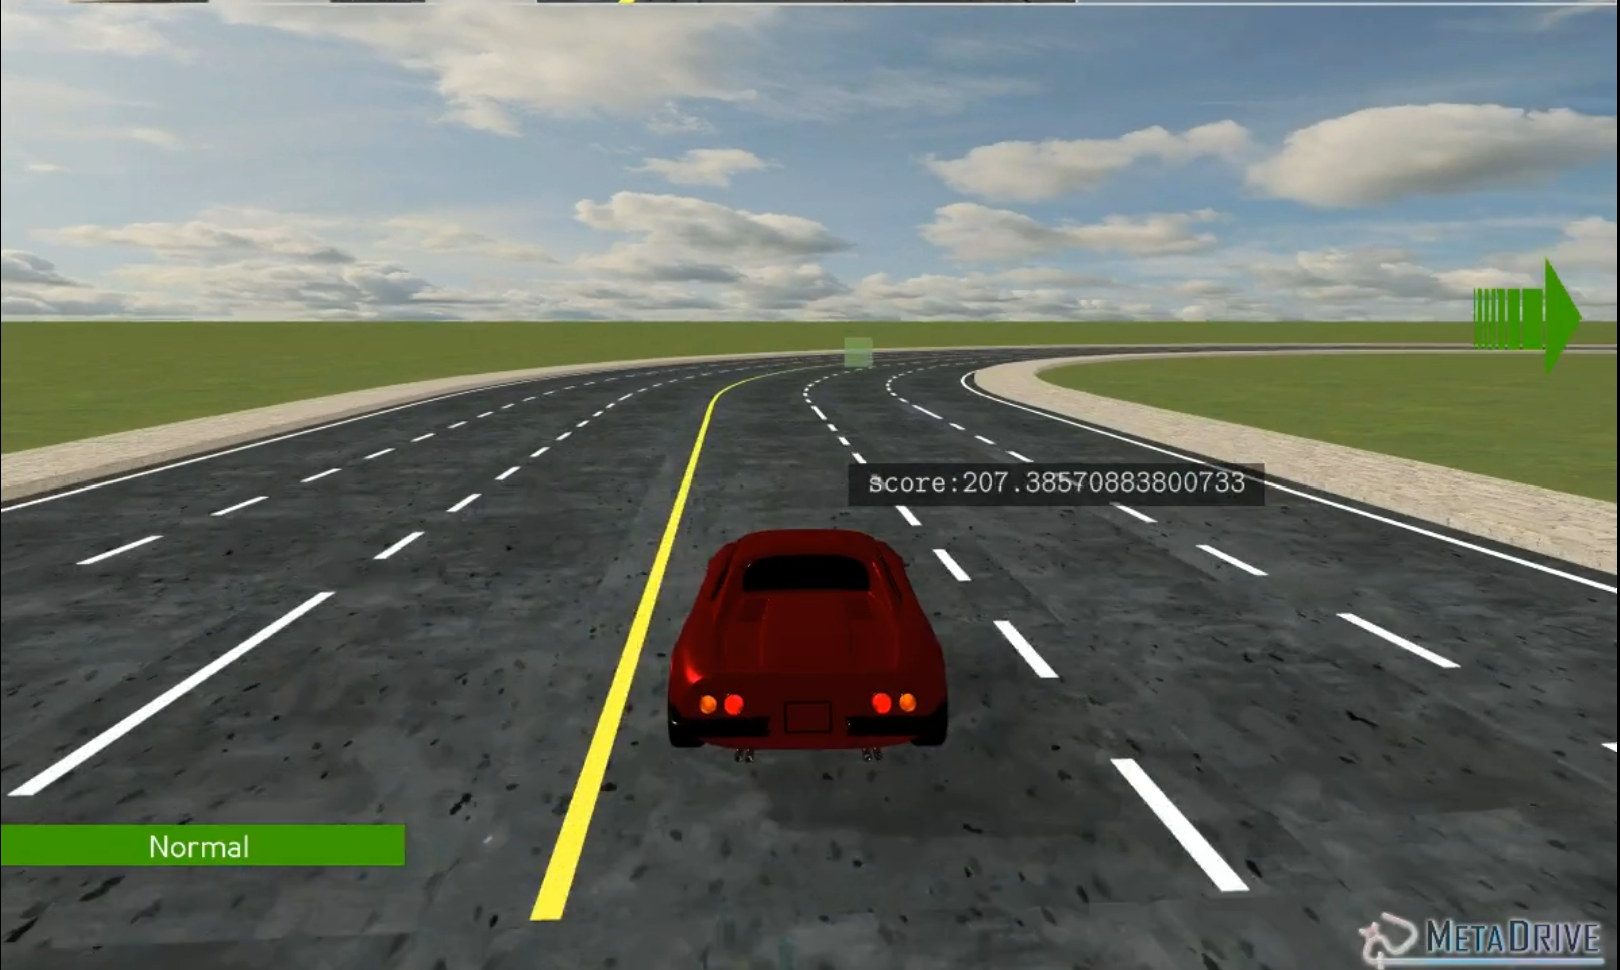
\includegraphics[width=0.3\textwidth]{images/chapter4/MetadriveVideoSc/7.png}
    }
    % \subfigure[]{
    % 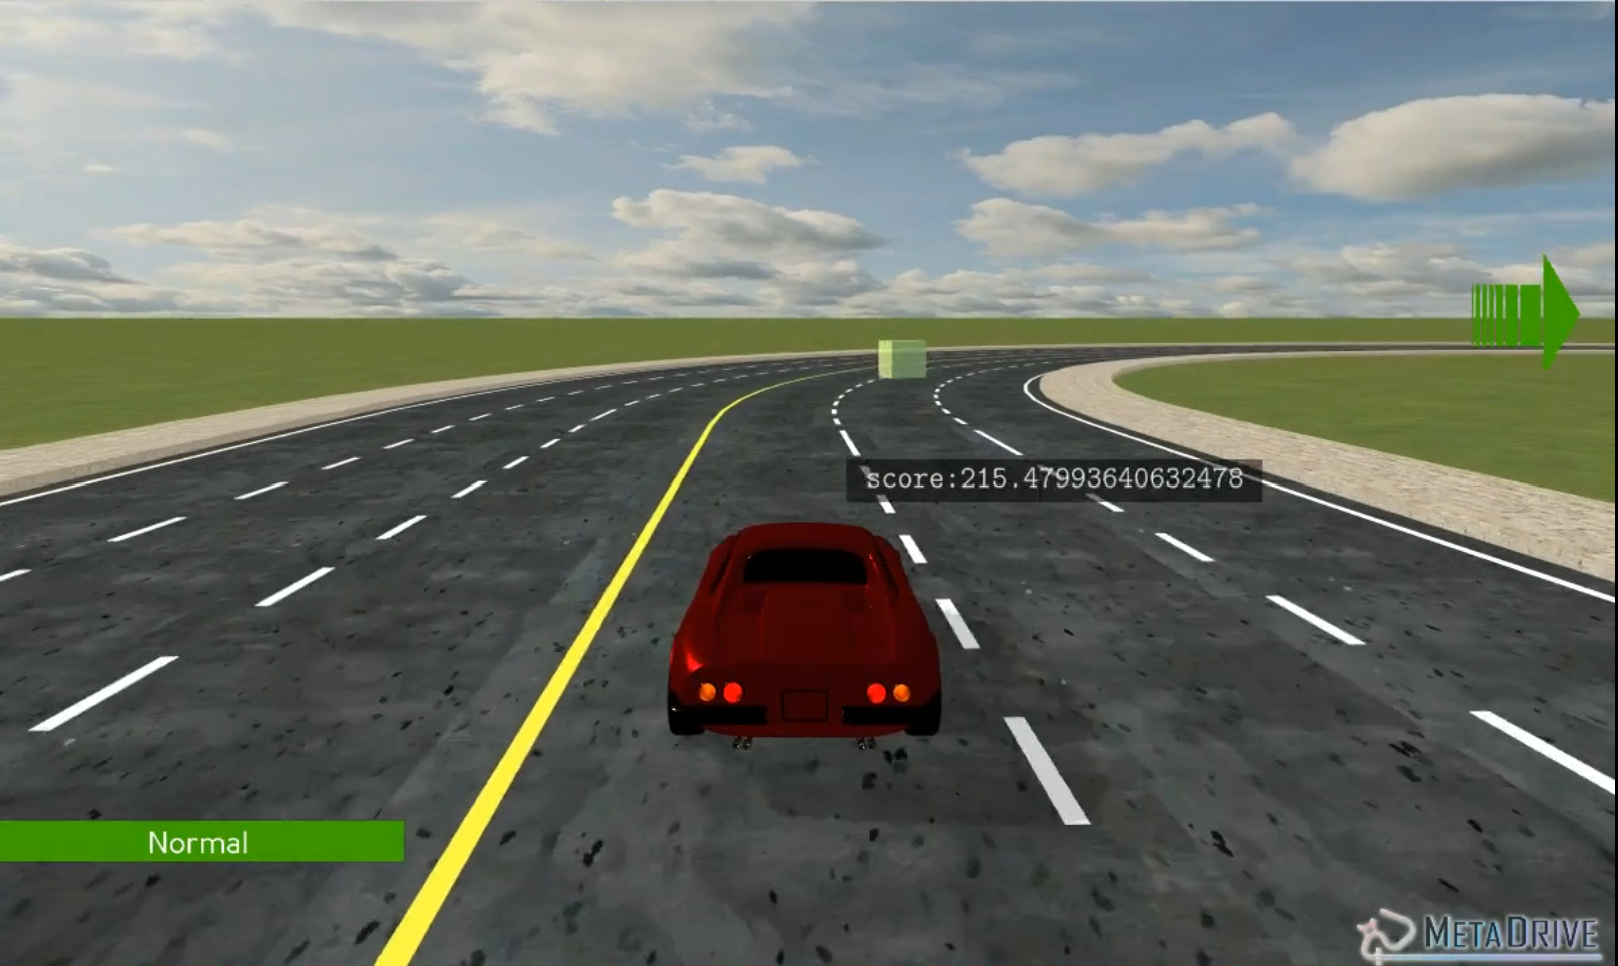
\includegraphics[width=0.2\textwidth]{images/chapter4/MetadriveVideoSc/8.png}
    % }
    \caption{基于DQN算法的控制器仿真效果}\label{基于DQN算法的控制器仿真效果} 
\end{figure}

以上行驶过程是智能体经过20000次训练达成的结果,经过20000次的训练,自动驾驶车辆基本学会了主动换道与循迹的策略,能够使自动驾驶车辆在一定的时间段内稳定行驶到终点。根据\ref{4.1基于DQN算法的决策器实验}节的结论,不再单独对DQN的输出结果进行分析,主要分析Double DQN和其他DQN算法的对比实验效果。

\subsubsection{基于DQN及其改进算法的控制器对比实验}

本实验验证了基于DQN、Double DQN和Dueling DQN算法的自动驾驶控制器,图\ref{metadriveQValue}和图\ref{metadriveLoss}表示了三种算法的收敛性对比,其中红、蓝、橙三色曲线分别代表DQN、Double DQN、Dueling DQN的输出收敛情况。

对于DQN和Double DQN:
\begin{equation}
    error = \frac{Loss}{Q\_Value} = \frac{0.3}{8.5} < 4\%
\end{equation}\label{dqn-controller-error}

对于Dueling DQN:
\begin{equation}
    error = \frac{Loss}{Q\_Value} = \frac{0.3}{3.5} < 10\%
\end{equation}\label{dueldqn-controller-error}

由于Dueling DQN输出的Q值相较于Double DQN和DQN算法过小,前者误差相对于后者较大,Dueling DQN的收敛程度较低,所以本节重点探究DQN和Double DQN的对比实验结果。

\begin{figure}[htbp]
    \vspace{13pt}
    \centering
    \subfigure[DQN及其改进算法的Q值输出]{
        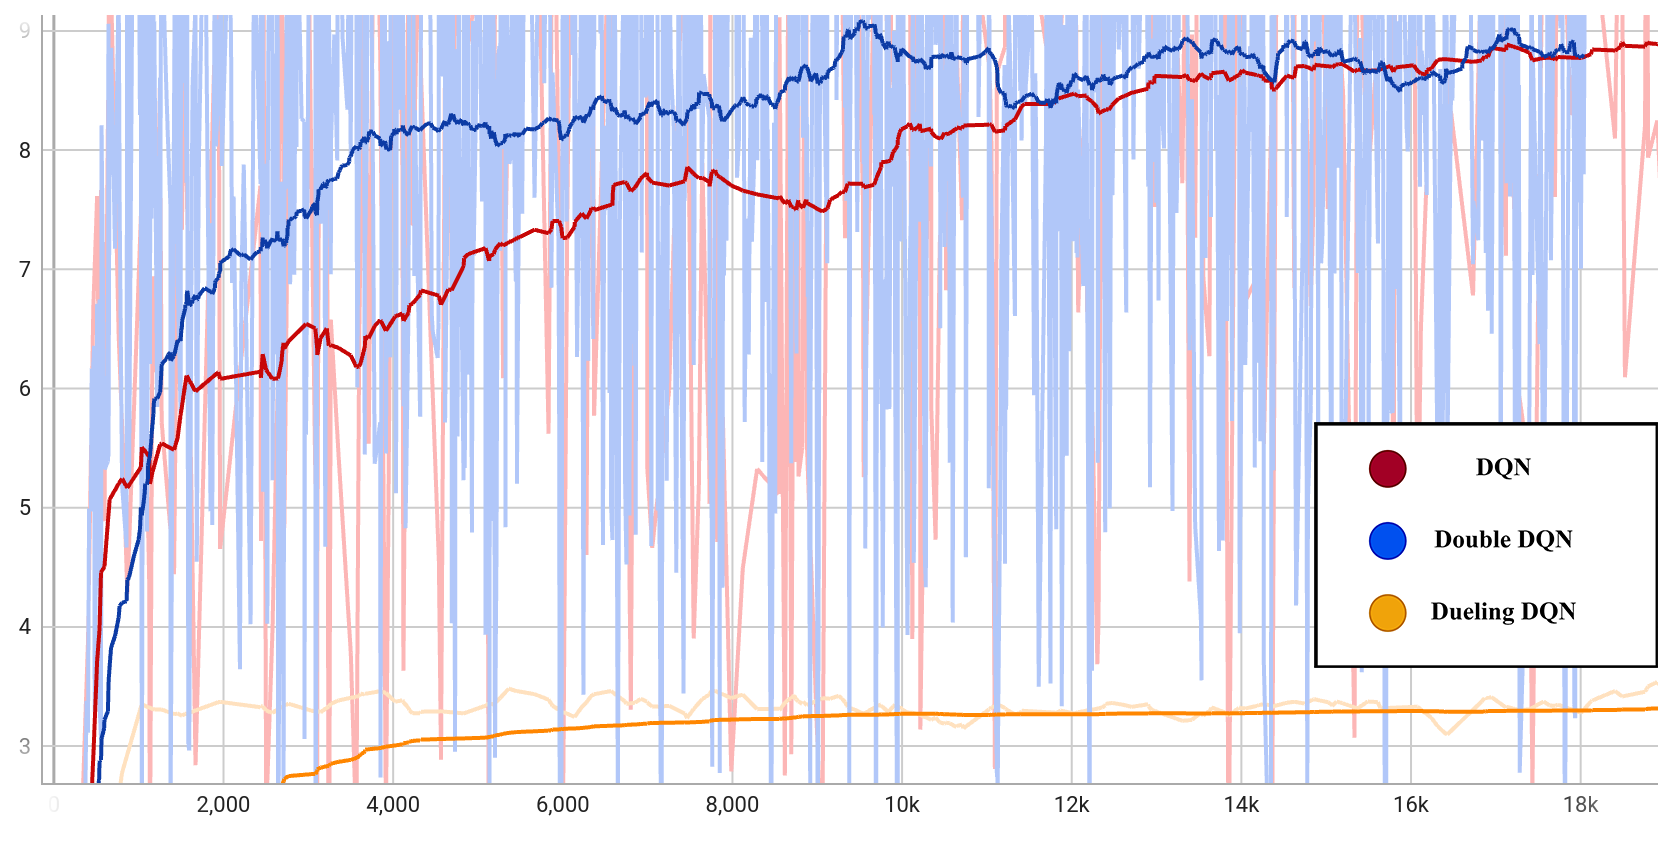
\includegraphics[width=0.45\textwidth]{images/chapter4/MetadrivePic/Q_Value.png}
        \label{metadriveQValue}
    }
    % \hspace{0.01in} % 两图片之间的距离
    \subfigure[DQN及其改进算法的损失函数]{
        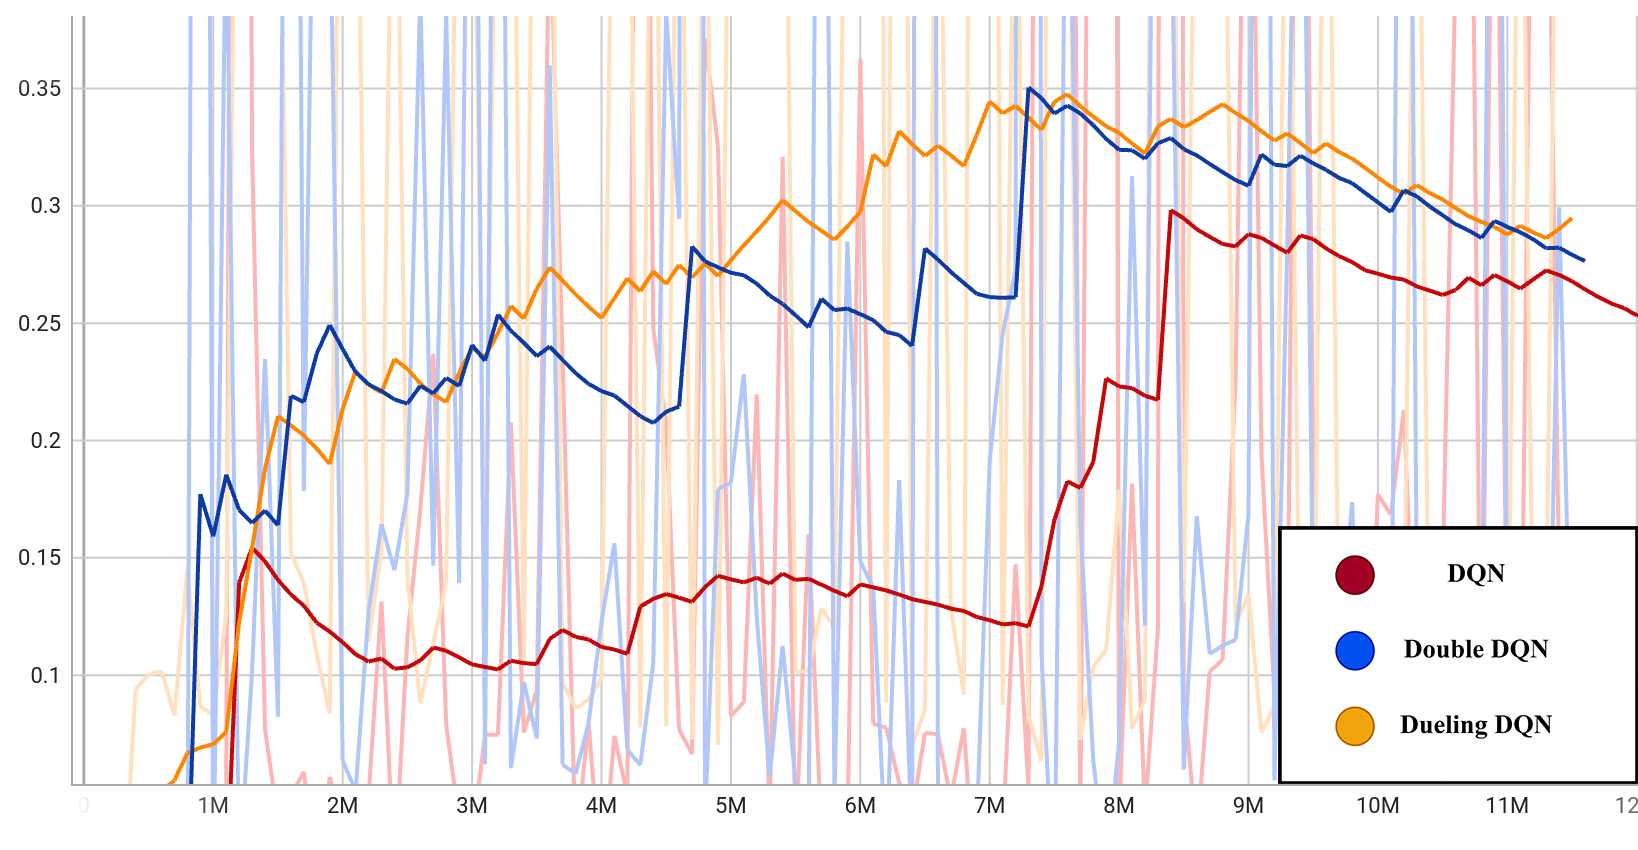
\includegraphics[width=0.45\textwidth]{images/chapter4/MetadrivePic/Loss.png}
        \label{metadriveLoss}
    }
    \subfigure[每回合奖励值输出]{
        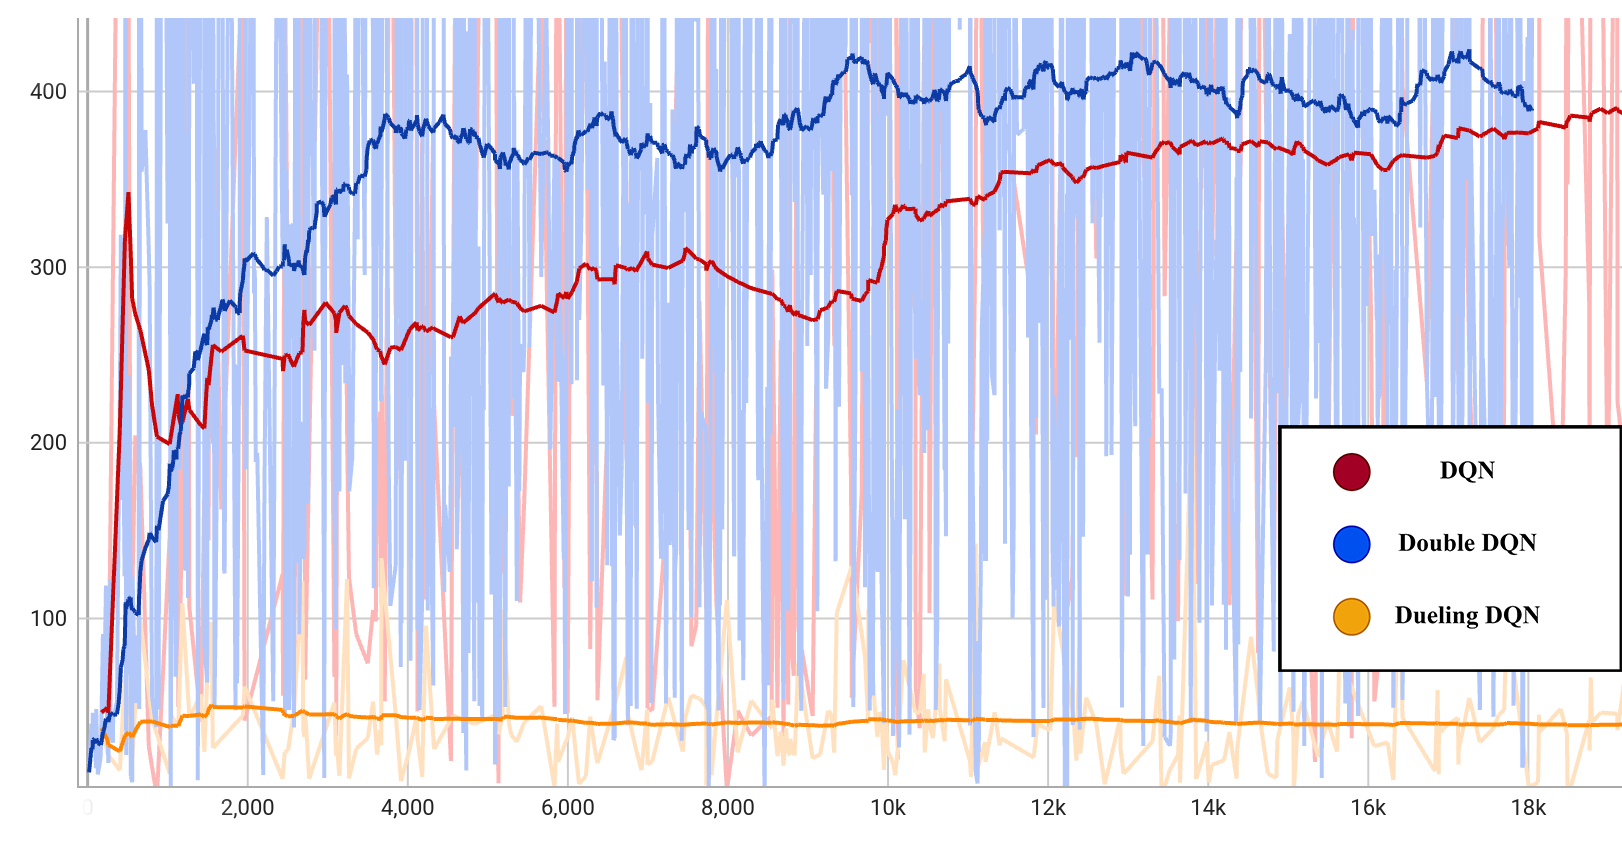
\includegraphics[width=0.45\textwidth]{images/chapter4/MetadrivePic/Ep_r.png}
        \label{metadriveEpr}
    }
    % \hspace{0.01in} % 两图片之间的距离
    \subfigure[平均动作奖励值输出]{
        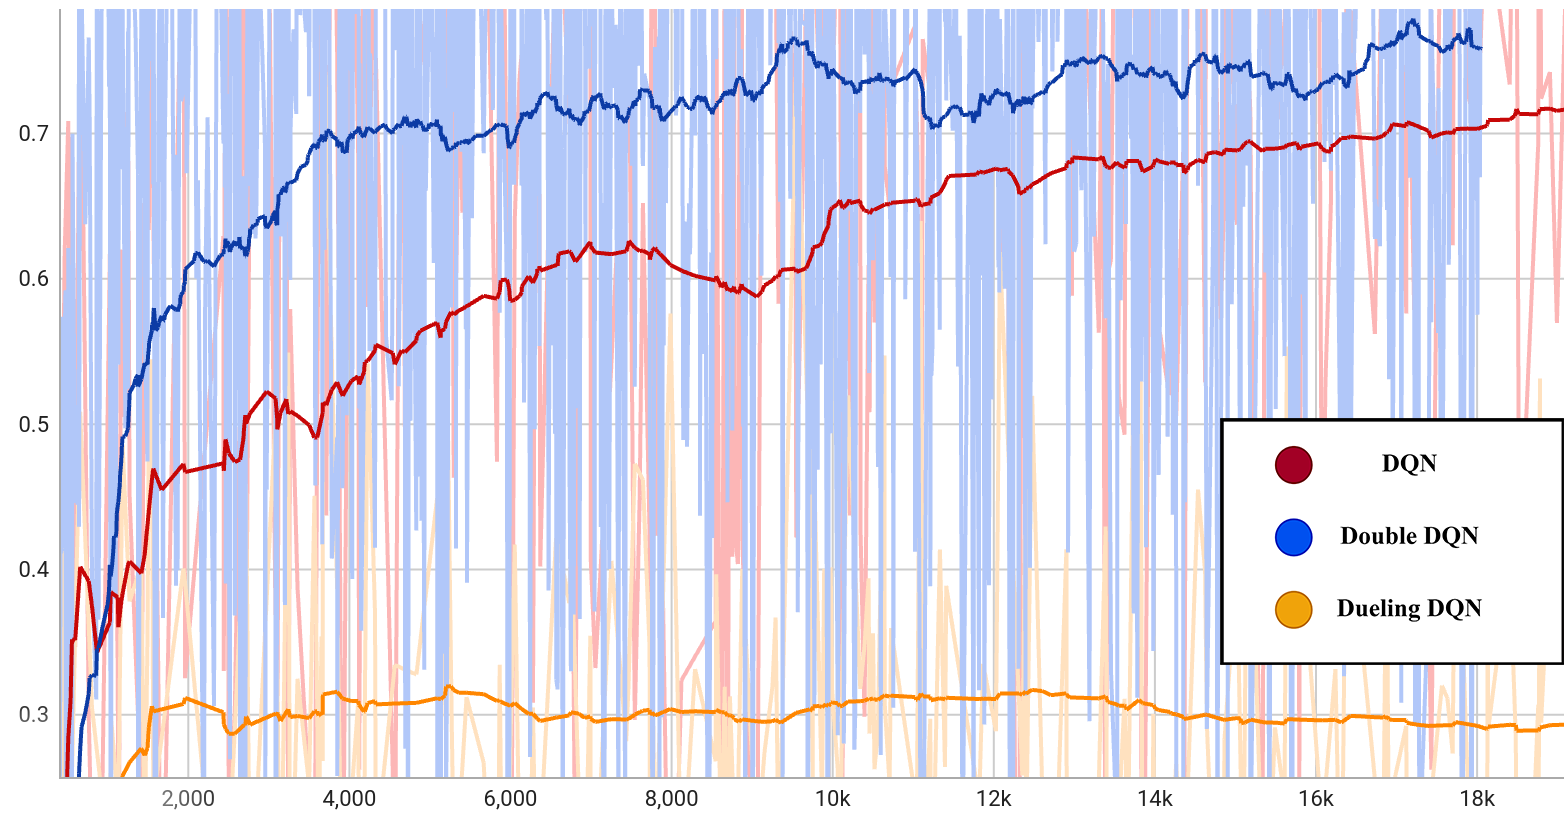
\includegraphics[width=0.45\textwidth]{images/chapter4/MetadrivePic/Ave_r.png}
        \label{metadriveAver}
    }
    \caption{DQN算法及其改进算法的控制器对比实验}\label{DQN算法及其改进算法的控制器对比实验} 
\end{figure}

由图\ref{metadriveEpr}和图\ref{metadriveAver}可知,Double DQN每回合得到的奖励值输出最高,平均动作奖励值也最高,这印证了\ref{4.1基于DQN算法的决策器实验}节中对Double DQN算法在动作选择和动作评估方面的分析,在更加复杂的环境中,Double DQN采取的网络参数更新策略避免选到被高估的次优行为,相对于最大化操作的值函数更新具有更加明显优势。

在\ref{4.1基于DQN算法的决策器实验}节中每回合奖励值输出函数最高的Dueling DQN算法在存在更加复杂输入的Metadrive仿真环境中表现不佳,一方面的原因是其两个支路所采用的全连接层结构较为简单,无法综合状态值函数$V(s)$和优势值函数$A(s,a)$使其满足自动驾驶车道保持和循迹的任务要求;另一方面的原因是其采用最大化操作的网络参数更新策略,存在选到被高估的次优行为的概率。

通过对以上仿真实验结果和数据的分析,DQN及其改进算法在Metadrive仿真实验环境中完成自动驾驶控制任务能够得到收敛,对于平均动作奖励和总体动作奖励,Double DQN能够得到相比于DQN和Dueling DQN更加良好的控制行为输出。

\section{本章小结}

本章根据第3章基于 DQN 算法的自动驾驶避障算法设计,进行了基于DQN及其改进算法的自动驾驶决策器和控制器实验,验证了基于DQN及其改进算法在自动驾驶决策器和控制器上的可行性和有效性。

针对自动驾驶决策器和控制器,Dueling DQN因其网络结构设计较为简单,在复杂性较低的自动驾驶决策仿真环境中表现较好,在复杂性较高的自动驾驶控制仿真环境中需要进一步改进网络结构。Double DQN因其在动作选择和动作评估上的参数更新改进,在两种仿真环境中都能够收敛,并且得到了相对于DQN和Dueling DQN更加良好的决策策略和控制行为输出。
